\documentclass[a4paper,11pt,oneside]{article}
\usepackage[utf8]{inputenc}
\usepackage[a4paper,top=3cm,bottom=3cm,left=3cm,right=3cm]{geometry}
\renewcommand{\familydefault}{\sfdefault}
\usepackage{helvet}
\usepackage[english]{babel}
\usepackage[style=numeric,language=english,sorting=none]{biblatex}
\usepackage{parskip}
\usepackage[margin=1cm]{caption}
\usepackage{booktabs}
\usepackage[pdftex]{graphicx}
\usepackage{subfigure}
\usepackage[pdftex]{hyperref}
\usepackage{amsmath}
\usepackage{amssymb}
\usepackage{array}
\usepackage{float} % make sure this is in your preamble


\usepackage{tikz}
\usetikzlibrary{arrows.meta, positioning}


\pdfadjustspacing=1

\newcommand{\mylastname}{Sah}
\newcommand{\myfirstname}{Sandip Kumar}
\newcommand{\mynumber}{5589263}
\newcommand{\myname}{\myfirstname{} \mylastname{}}
% \newcommand{\mytitle}{A fast implementation of deep neural-network potentials for molecular dynamics simulations of alloys}
\newcommand{\mytitle}{Accurate implementation of DeepMD-v2 potential calculation in HALMD for single species, extension to multi-species and Automatic-Differentiation-Based Force Computation}
\newcommand{\mysupervisor}{Prof. Dr. Felix Höfling}

\hypersetup{
  pdfauthor = {\myname},
  pdftitle = {\mytitle},
  colorlinks = {true},
  linkcolor = {black}
}

\addbibresource{references.bib}

\begin{document}
\pagenumbering{roman}
\thispagestyle{empty}

\begin{flushright}
  \includegraphics[width=0.35\textwidth]{./images/fub_logo_2.svg.png}
\end{flushright}
\vspace{10mm}

\vspace*{40mm}
\begin{center}
  \huge
  \textbf{\mytitle}
\end{center}
\vspace*{4mm}
\begin{center}
  \Large by
\end{center}
\vspace*{4mm}
\begin{center}
  \LARGE
  \textbf{\myname}
\end{center}
\vspace*{20mm}
\begin{center}
  \Large
  Master thesis in computational science
\end{center}
\vfill
\begin{flushleft}
  \large
  Submission: {09 January 2026} \hfill Supervisor: \mysupervisor \\
  \rule{\textwidth}{1pt}
\end{flushleft}
\begin{center}
  Freie Universität Berlin $|$ Department of Mathematics and Computer Science\\
  Institute of Mathematics
\end{center}

\newpage
\thispagestyle{empty}

\begin{center}
  \Large \textbf{Statutory Declaration}
  \vspace*{8mm}
\end{center}

\begin{center}
\begin{tabular}{lp{85mm}}
    \hline
    Family Name, Given/First Name & \mylastname, \myfirstname \\
    Matriculation number          & \mynumber                 \\
    Kind of thesis submitted      & Master Thesis             \\
    \hline
  \end{tabular}
  \vspace*{8mm}
\end{center}



% \section*{Declaration of Authorship}



% I hereby confirm that I have completed this thesis independently and without the use of sources and
% aids other than those specified. This thesis has not been submitted in the same or a similar form as an
% examination at any other university.

% I have identified all quotations, both direct and indirect, as such. Literal quotations have been marked
% with quotation marks (“...”). I have also cited Internet sources used, stating their full address and the
% time of last access.

% I take note:

% I am obliged to comply with the rules of good scientific practice. Violations will be subject to
% disciplinary action. In particular, attempts to cheat will automatically be assessed as “fail” (5.0)
% (§ 19 (3) sentence 1 RSPO). The adoption of external ideas / results / concepts etc. without
% appropriate identification (plagiarism) is generally an attempt to deceive. Depending on the severity,
% further sanctions are possible up to the final failure of the examination and thus the degree program
% (§ 19 (3) sentence 3 and 4 RSPO).

% The grade may be lowered (including a failing grade) due to a lack of independence if a significant
% amount of other persons' explanations are copied, even if they are identified as such and no attempt to
% deceive has been made.


% Following operations were performed in my thesis using generative AI:


% \begin{center}
% \begin{tabular}{|p{7cm}|p{5cm}|}
% \hline
% \textbf{Type and location of AI assistance} & \textbf{AI tool used} \\
% \hline
% Paraphrasing of section Introduction and Background
% & ChatGPT~4.0 \\
% \hline
% Summarizing overview of methodology
% & ChatGPT~4.0 \\
% \hline
% Formula Organizaation inside sector Force Computation
% & ChatGPT~4.0 \\
% \hline
% Linguistic correction of the entire text
% & Grammarly \\
% \hline
% \end{tabular}
% \end{center}


% \bigskip

% I understand that using AI-generated text or other content does not guarantee its quality. I take full
% responsibility for all machine-generated content that I use and am liable for any errors, distortions,
% or incorrect references, as well as any violations of data protection, copyright law, or plagiarism.
% Furthermore, I assure you that my editorial influence prevails in this work.

% I confirm that I did not use any AI-based tools prohibited by the examination regulations.

% \vspace{1.5cm}

% \noindent
% Date:\hfill Signature:

\section*{Declaration of Authorship}

I hereby declare that I have completed this thesis independently and that I have not used any sources
or aids other than those explicitly stated. This thesis has not been submitted, in whole or in part, to
any other university for the purpose of obtaining a degree.

All direct and indirect quotations have been clearly identified. Sources from the internet have been
properly cited.

I am aware of the rules of good scientific practice and understand that violations, in particular
plagiarism or misrepresentation of authorship, may lead to disciplinary consequences, including the
failure of the thesis.

The following forms of generative AI assistance were used in the preparation of this thesis:

\begin{center}
\begin{tabular}{|p{7cm}|p{5cm}|}
\hline
\textbf{Type of AI assistance} & \textbf{AI tool used} \\
\hline
Paraphrasing of Introduction and Background sections
& ChatGPT~4.0 \\
\hline
Summarizing methodological descriptions
& ChatGPT~4.0 \\
\hline
Assistance with formula organization in the force computation section
& ChatGPT~4.0 \\
\hline
Linguistic proof reading of the full manuscript
& Grammarly \\
\hline
\end{tabular}
\end{center}

I take full responsibility for all AI-assisted content included in this thesis and confirm that its use
complies with the applicable examination regulations. My own academic judgment and editorial control
were maintained throughout the work.

\vspace{1.2cm}

\noindent
Date:\hfill Signature:


% \section*{Eigenständigkeitserklärung}

% Hiermit erkläre ich, dass ich die vorliegende Arbeit selbstständig und ohne unerlaubte Hilfe
% angefertigt habe. Es wurden keine anderen als die angegebenen Quellen und Hilfsmittel verwendet.
% Diese Arbeit wurde weder vollständig noch in Teilen an einer anderen Hochschule als
% Prüfungsleistung eingereicht.

% Alle wörtlichen und sinngemäßen Zitate sind als solche kenntlich gemacht. Verwendete Internetquellen
% wurden ordnungsgemäß angegeben.

% Ich bin mir der Regeln guter wissenschaftlicher Praxis bewusst und weiß, dass Verstöße, insbesondere
% Plagiate oder falsche Angaben zur Urheberschaft, zu disziplinarischen Maßnahmen bis hin zum
% Nichtbestehen der Arbeit führen können.

% Im Rahmen der Erstellung dieser Arbeit wurden folgende Formen generativer KI-Unterstützung
% verwendet:

% \begin{center}
% \begin{tabular}{|p{7cm}|p{5cm}|}
% \hline
% \textbf{Art der KI-Unterstützung} & \textbf{Verwendetes KI-Werkzeug} \\
% \hline
% Paraphrasierung der Abschnitte Einleitung und Hintergrund
% & ChatGPT~4.0 \\
% \hline
% Zusammenfassende Darstellung der Methodik
% & ChatGPT~4.0 \\
% \hline
% Unterstützung bei der Strukturierung von Formeln im Abschnitt zur Kraftberechnung
% & ChatGPT~4.0 \\
% \hline
% Sprachliche Überarbeitung des gesamten Textes
% & Grammarly \\
% \hline
% \end{tabular}
% \end{center}

% Ich übernehme die volle Verantwortung für alle mit Hilfe von KI erstellten oder überarbeiteten Inhalte
% und versichere, dass deren Nutzung den geltenden Prüfungsordnungen entspricht. Die inhaltliche
% Kontrolle und wissenschaftliche Bewertung lagen jederzeit bei mir.

% \vspace{1.2cm}

% \noindent
% Ort, Datum:\hfill Unterschrift:




\newpage

\section*{Abstract}
% A concise 200–300 word summary of:
% \begin{itemize}
%   \item Motivation (accelerating atomistic simulations using neural network potentials)
%   \item Goal (integrating DeepMD potential calculation into HALMD)
%   \item Method (extracting weights, replicating inference in C++/CUDA)
%   \item Key results and performance (accuracy vs. speed trade-off)
%   \item Conclusions
% \end{itemize}

\newpage
\setcounter{tocdepth}{2}
\tableofcontents
\clearpage
\pagenumbering{arabic}

% ===============================


\section{Introduction}

\subsection{Motivation}

Molecular dynamics (MD) simulations play a central role in materials science by
providing atomistic insight into the behavior of complex systems across a wide
range of length and time scales. In MD, atomic trajectories are obtained by
integrating Newton’s equations of motion using forces derived from an
interatomic potential that approximates the underlying quantum-mechanical
potential energy surface (PES) \cite{frenkel2023understanding}.

Classical empirical interatomic potentials—such as Lennard--Jones, embedded-atom
method (EAM), and bond-order potentials—are computationally efficient and allow
simulations involving millions of atoms over nanoseconds to microseconds
\cite{daw1984eam,brenner2002reactive}. However, these models rely on fixed
analytical functional forms and limited parameter sets, which makes them too
rigid to accurately describe complex bonding environments involving bond
breaking and formation, charge transfer, polarization effects, defect chemistry,
and chemically heterogeneous systems \cite{behler2007generalized,thompson2015spectral}.
% For example, EAM potentials accurately reproduce bulk metallic cohesion but often
% fail for surface reactions and defect energetics \cite{daw1984eam}, while
% reactive bond-order potentials such as REBO suffer from limited transferability
% across different chemical environments \cite{brenner2002reactive}.

At the other end of the spectrum, \textit{ab initio} methods compute forces
directly from quantum mechanics by explicitly solving the electronic structure
problem, typically within density functional theory (DFT)
\cite{kohn1965self,hohenberg1964inhomogeneous}. These approaches provide highly
accurate predictions of bonding, reaction pathways, and material properties
\cite{marx2009ab}. However, their computational cost scales steeply with
system size—typically as $\mathcal{O}(N^3)$ with the number of electrons—which
restricts practical simulations to at most a few thousand atoms and time scales
of tens to hundreds of picoseconds \cite{marx2009ab}.

Machine-learned interatomic potentials overcome this long-standing accuracy–efficiency
dilemma. By training flexible models, particularly deep neural networks, on large
datasets of \textit{ab initio} reference calculations, these potentials learn the
PES without imposing restrictive analytical forms \cite{behler2007generalized,noe2020mlreview}.
As a result, modern neural network potentials achieve energy errors on the order
of a few meV/atom and force errors of tens of meV/\AA, which is comparable to the
intrinsic accuracy of DFT \cite{bartok2015gap,schutt2017schnet,batzner20223}.
At the same time, their evaluation cost scales linearly with system size and can
be efficiently executed on GPUs, enabling simulations with millions of atoms at
computational cost comparable to classical MD
\cite{wang2018deepmd,zeng2023deepmdv2}. This combination of near--quantum mechanical
accuracy and classical-MD performance has made machine-learned potentials a
transformative technology for large-scale materials modeling.

The work by Andrés Cruz, titled \textit{``Deep Neural Networks Potentials for
Scalable Molecular Dynamics Simulations on Accelerator Hardware''}
\cite{cruz2025deepmd}, represents an important step toward integrating Deep
Potential models into the high-performance GPU-accelerated simulation engine
HALMD. His work reconstructs the DeePMD-kit inference pipeline inside HALMD,
extracts network weights from trained TensorFlow models, and compute energy and
force predictions for a \textit{single-species copper system} \cite{Cu_fcc_slabs_2023}.
In particular, his implementation focuses on the two-body embedding smooth edition
(DeepPot-SE) descriptor and reproduces the filter and fitting networks only for a
monoatomic system, making it suitable for single-element metals.

However, the implementation in \cite{cruz2025deepmd} remains limited to the
simplest class of DeepMD-v2 architectures and does not include multi-species
support. Several essential components of the full DeepMD-v2 computational graph
are simplified or omitted.

This thesis builds directly on the work of Cruz \cite{cruz2025deepmd} and advances
it substantially. The primary contributions of the present work are:
\begin{enumerate}
    \item Generalizing the HALMD Deep Potential integration to \textit{multi-species,
          multi-body DeepMD-v2 models}, enabling simulations of binary and
          multicomponent alloy systems.
    \item Reconstructing descriptor and fitting networks for the full
          \textit{multi-species DeepPot-SE architecture}, including multi-body
          descriptor terms.
    \item Improving the numerical \textit{accuracy} of the HALMD implementation by
          incorporating essential computational steps missing in the previous
          work, including proper cutoff normalization and multi-species descriptor
          algebra.
\end{enumerate}

Through these extensions, the present thesis transforms HALMD from supporting a
prototype single-component DeepMD potential into a \textit{high-accuracy,
multi-species DeepMD-v2 engine}, significantly broadening its applicability and
enabling large-scale molecular dynamics simulations of 
multicomponent materials at near--quantum mechanical accuracy.

Despite the significant progress achieved by recent machine-learning-based
interatomic potentials and the integration of DeepMD into HALMD by
Cruz \cite{cruz2025deepmd}, a substantial gap remains between
state-of-the-art DeepMD models and their practical deployment within large-scale
GPU-accelerated molecular dynamics engines. In particular, the lack of full
multi-species support and the omission of several critical components of the
DeepMD-v2 inference pipeline currently prevent HALMD from exploiting the full
predictive power of modern DeepMD models for chemically complex materials.
% Bridging this gap is essential for enabling high-fidelity simulations of
% realistic multicomponent systems at scale.

\subsection{Objectives and scope}

Motivated by this gap, the objective of this thesis is to extend and generalize the
Deep Potential (DeePot) implementation in HALMD beyond the single-species, two-body
descriptor developed by Cruz \cite{cruz2025deepmd}. While Cruz's work successfully
demonstrated that HALMD can evaluate a DeePMD-v2 model for a monoatomic copper system,
several components required for full multi-species DeepMD-v2 inference were missing.
Most notably, the previous implementation did not include (i) the periodic coordinate
extension and neighbor-list construction used in DeepMD \cite{wang2018deepmd},
(ii) normalization and scaling layers defined in the DeePMD-v2 framework
\cite{zeng2023deepmdv2}, (iii) species-dependent descriptors, or (iv) descriptor
and filter weights that depend simultaneously on the central and neighbor species,
as introduced in the multi-species DeepPot-SE descriptor \cite{zeng2023deepmdv2}.

This thesis addresses these limitations by implementing the complete multi-species
DeepMD-v2 inference pipeline, including accurate periodic handling of atomic environments.
Specifically, the thesis pursues the following objectives:

\begin{enumerate}

    \item \textbf{Implement coordinate normalization, ghost-cell extension, and multi-type neighbor list construction.}
    The previous implementation did not include the canonical DeePMD preprocessing steps
    for periodic systems---wrapping coordinates into the primary simulation cell, generating
    ghost atoms to cover the cutoff radius, and constructing species-grouped neighbor
    lists---as described in the DeePMD methodology \cite{wang2018deepmd, zeng2023deepmdv2}.
    Implementing these steps ensures that HALMD reproduces the correct local environments
    required by the DeepPot-SE descriptors under periodic boundary conditions.

    \item \textbf{Implement species-dependent filter networks.}
    Extend the single-species embedding and filter networks used in \cite{cruz2025deepmd}
    to support arbitrary numbers of atomic types, following the species-indexed filter
    network formulation defined in the DP-v2 architecture \cite{zeng2023deepmdv2}.

    \item \textbf{Reproduce the full DeepMD-v2 inference procedure with higher accuracy.}
    Incorporate several computational steps omitted in previous work, including normalization
    layers, descriptor scaling operations, smooth cutoff functions, and full force
    backpropagation through descriptor derivatives, consistent with the DeepMD-v2
    formulation \cite{zeng2023deepmdv2, wang2018deepmd}.

\end{enumerate}

\noindent\textbf{Scope:}
This thesis focuses exclusively on the inference stage of DeepMD-v2, i.e., the computation
of energies and forces from pre-trained models. Model training is outside the scope of this
work. The implementation targets the multi-species DeepPot-SE descriptor and does not cover
other descriptor families such as end-to-end or message-passing potentials. The work provides
support for multi-species atomic systems relevant to alloys and chemically complex materials,
while the underlying molecular dynamics algorithms (integrators, thermostats, barostats) rely
on HALMD's existing infrastructure.

\newpage


\section{Background}


% \subsection{Ab initio molecular dynamics (AIMD) and Car--Parrinello molecular dynamics (CPMD)}


\subsection{Ab initio molecular dynamics (AIMD) and Car--Parrinello molecular dynamics (CPMD)}

Ab initio molecular dynamics (AIMD) comprises a class of simulation methods in which
interatomic forces are obtained directly from quantum-mechanical calculations of the
electronic structure, rather than from predefined empirical or semi-empirical interatomic
potentials \cite{marx2009ab,car1985unified}. In contrast to classical molecular
dynamics, where the potential energy surface (PES) is approximated by analytical
expressions with fixed parameters, AIMD evaluates the PES explicitly from first
principles at every molecular dynamics time step.

In practice, this means that for each atomic configuration the electronic Schr\"odinger
equation is solved approximately using electronic structure methods, most commonly
density functional theory (DFT) \cite{kohn1965self,hohenberg1964inhomogeneous}.
The resulting electronic ground-state energy defines the instantaneous value of the PES,
and its gradient with respect to nuclear coordinates yields the forces acting on the atoms.
Because the electronic structure is recomputed \emph{on-the-fly} during the simulation,
AIMD naturally incorporates changes in chemical bonding, charge redistribution,
polarization effects, and many-body interactions without requiring any predefined bonding
topology or fitted potential parameters \cite{marx2009ab}.

In the most direct formulation of AIMD, known as Born--Oppenheimer molecular dynamics
(BOMD), the electronic ground state is determined independently at every molecular
dynamics step for the current atomic geometry. For a fixed nuclear configuration, the
electronic structure problem is solved iteratively using a self-consistent field (SCF)
procedure: starting from an initial guess for the electronic density, the Kohn--Sham
equations of DFT are solved repeatedly until the input and output densities converge and
the Kohn--Sham energy functional reaches a minimum subject to the orthonormality of
the electronic orbitals \cite{payne1992iterative,marx2009ab}. Once convergence is
achieved, the forces on the nuclei are obtained from the gradient of the converged
electronic energy, and the atomic positions are advanced according to Newton’s
equations of motion. Although this procedure yields highly accurate forces, the need to
perform a full SCF optimization at every time step makes BOMD computationally
expensive.

Car--Parrinello molecular dynamics (CPMD) provides an alternative formulation of AIMD
that avoids explicit electronic energy minimization at each step \cite{car1985unified}.
CPMD introduces an extended Lagrangian in which both the nuclear coordinates and the
Kohn--Sham orbitals are treated as dynamical variables. The electronic degrees of freedom
are assigned a fictitious mass and propagated alongside the nuclei, while constraints
maintain the orthonormality of the electronic orbitals. If the fictitious electronic mass is
chosen sufficiently small, the electronic subsystem remains adiabatically separated from
the nuclear motion and stays close to the instantaneous Born--Oppenheimer surface,
thereby reproducing ground-state forces without performing a full SCF optimization at
every time step \cite{marx2009ab}.

In CPMD, nuclear motion follows classical Newtonian dynamics, whereas the electronic
orbitals evolve according to equations of motion derived from the Kohn--Sham energy
functional. This unified dynamical treatment significantly reduces the computational
cost per time step compared to BOMD, while maintaining forces consistent with first-
principles electronic structure. Nevertheless, CPMD remains computationally demanding
because each step still requires evaluating the Kohn--Sham Hamiltonian, performing
large-scale matrix operations, and maintaining orthonormality of the electronic states.
As a result, practical simulations are typically limited to system sizes of at most a few
hundred atoms and time scales on the order of tens to hundreds of picoseconds
\cite{marx2009ab,giannozzi2009quantum}.

Consequently, CPMD is primarily employed as a high-accuracy reference method rather
than as a routine tool for large-scale molecular dynamics simulations. Its predictive power
arises from its explicit treatment of the electronic structure, which allows it to describe
chemical reactions, diffusion mechanisms, and charge-transfer processes from first
principles. For example, Zhong \textit{et al.} \cite{zhong2025hydrogen} used CPMD to
investigate hydrogen diffusion in complex garnet electrolytes, accurately resolving
hydrogen migration pathways and energy barriers that are difficult to capture with
empirical force fields. At the same time, their study highlights the inherent limitations of
CPMD: the high computational cost restricts the accessible length and time scales, making
it impossible to directly simulate macroscopic diffusion processes or long-term structural
evolution. These limitations motivate the development of machine-learned interatomic
potentials that reproduce first-principles accuracy at a fraction of the computational cost.


\subsection{High-accuracy large-scale molecular dynamics (HALMD) software}

HALMD package is a high-performance, open-source molecular dynamics simulation framework designed for large-scale studies
of condensed matter systems. HALMD is built around a modular C++ architecture with a
strong emphasis on numerical precision, extensibility, and efficient parallel execution
on graphics processing units (GPUs) \cite{colberg2011highly}. It provides the
computational infrastructure required to simulate systems containing millions of
particles over long physical time scales.

HALMD employs the classical molecular dynamics approach, in which atomic motion is
governed by Newton’s equations of motion,

\begin{equation}
   m_i \frac{d^2 \mathbf{r}_i}{dt^2}
    = - \nabla_i U(\mathbf{r}_1, \mathbf{r}_2, \ldots, \mathbf{r}_N), 
\end{equation}

where the potential energy function \( U \) describes interatomic interactions. In
standard applications, \( U \) is given by analytical or tabulated empirical potentials,
such as the Lennard--Jones, Gaussian Core, or Yukawa models. While these classical empirical 
models are computationally efficient and enable
simulations of very large systems over long time scales, numerous studies have shown
that they often fail to reproduce important quantum-mechanical effects such as bond
breaking and formation, charge transfer, polarization, and accurate reaction barriers.
For example, Daw and Baskes demonstrated that embedded-atom method (EAM) potentials
can accurately describe bulk metallic cohesion but struggle for defect energetics and
chemical reactions \cite{daw1984eam}. Similarly, Brenner \textit{et al.} showed that
reactive empirical bond-order (REBO) potentials capture many covalent bonding trends
but remain limited in transferability across chemical environments \cite{brenner2002reactive}.
In contrast, first-principles methods such as CPMD explicitly resolve the electronic
structure and have been shown to accurately predict reaction mechanisms, diffusion
pathways, and defect energetics in complex materials \cite{marx2009ab,car1985unified}.


A defining strength of HALMD is its GPU-accelerated backend. Computationally intensive
tasks, including force evaluation, neighbor-list construction, and time integration,
are implemented using NVIDIA CUDA and, more recently, SYCL to support heterogeneous
computing platforms \cite{colberg2011highly,halmdGithub}. Spatial domain decomposition
and cell-based neighbor lists enable efficient scaling on multi-GPU systems, achieving
orders-of-magnitude speedups compared to CPU-only implementations.

HALMD follows a modular design philosophy in which integrators, interaction potentials,
neighbor-list builders, and observables are implemented as interchangeable components
configured via a Lua scripting interface \cite{halmdManual}. This modularity allows new
force models to be integrated without modification of the core simulation engine.
Simulation data are stored in the H5MD format \cite{debuyl2014h5md}, a standardized,
self-describing file format for molecular dynamics data built on top of the HDF5
hierarchical data model. H5MD organizes simulation output—such as particle positions,
velocities, forces, energies, and observables—into a structured hierarchy with explicit
metadata describing units, physical meaning, and simulation parameters. This design
ensures portability across simulation codes, long-term data reproducibility, and direct
compatibility with modern analysis and visualization tools, thereby facilitating
post-processing, data sharing, and workflow automation.


In this thesis, HALMD serves as the computational backbone for large-scale molecular
dynamics simulations. By replacing conventional empirical interaction potentials with
machine-learned DeepMD-v2 force fields, HALMD becomes capable of performing simulations
with near \textit{ab initio} accuracy at classical MD computational cost. The integration
of a full multi-species DeepMD-v2 inference pipeline into HALMD thus bridges the gap
between the accuracy of CPMD and the scalability required for practical materials
modeling.

% \subsection{HALMD Software}

% The High-Accuracy Large-scale Molecular Dynamics (HALMD) package is a high-performance, open-source molecular dynamics (MD) simulation framework designed to study the microscopic dynamics of liquids, glasses, and other condensed matter systems. HALMD is built around a modular C++ architecture with a strong emphasis on numerical precision, extensibility, and efficient parallel computation on graphics processing units (GPUs) \cite{colberg2011highly}. It provides a versatile platform for conducting large-scale classical molecular dynamics simulations involving millions of particles.

% HALMD employs the \textit{classical molecular dynamics} approach, in which atomic motion is governed by Newton’s equations of motion,
% \[
% m_i \frac{d^2 \mathbf{r}_i}{dt^2}
% = - \nabla_i U(\mathbf{r}_1, \mathbf{r}_2, \ldots, \mathbf{r}_N),
% \]
% where \( U \) is a predefined analytical potential describing interatomic interactions. The accuracy of a classical MD simulation depends on the accuracy of this potential. HALMD supports several built-in empirical pair potentials, such as Lennard–Jones, Gaussian Core, and Yukawa models, and additionally allows users to supply tabulated pair potentials. These empirical models do not involve quantum-mechanical calculations and thus differ from \textit{ab initio} molecular dynamics (AIMD), where forces are computed directly from electronic structure methods.

% One of HALMD’s defining strengths is its high-performance GPU backend. The software employs NVIDIA’s CUDA to accelerate computationally intensive tasks such as force evaluation, neighbor-list construction, and time integration \cite{colberg2011highly}, and more recent versions extend support to heterogeneous computing platforms through SYCL \cite{halmdGithub}. Spatial domain decomposition and cell binning enable efficient scaling on multi-GPU systems, achieving orders-of-magnitude speedups compared to CPU-only implementations. HALMD also supports mixed-precision arithmetic, selectively applying double precision to critical operations to ensure long-term numerical stability without compromising performance.

% HALMD follows a modular design philosophy. Core components—integrators, interaction potentials, neighbor-list builders, and observables—are implemented as interchangeable modules configurable through a Lua scripting interface \cite{halmdManual}. This modularity makes it straightforward to extend HALMD with new functionality, including custom potentials, analysis routines, and data exporters. Simulation data are stored in the H5MD format \cite{debuyl2014h5md}, an HDF5-based standard widely supported by analysis tools in computational physics and chemistry.

% These characteristics make HALMD an ideal platform for integrating machine-learned interatomic potentials. Its GPU-accelerated, modular architecture provides the necessary infrastructure to replace conventional analytical potentials with neural-network-based force fields. In this thesis, HALMD serves as the host MD engine into which the Deep Potential Molecular Dynamics (DeepMD) model is embedded. The goal is to achieve \textit{ab initio}-level accuracy within HALMD’s efficient large-scale simulation framework by implementing a full multi-species DeepMD-v2 inference pipeline.




\subsection{Neural network potential (NNP)}

% In recent years, machine learning techniques—particularly deep neural networks (DNNs) have revolutionized the construction of interatomic potentials for molecular dynamics simulations. Traditional analytical potentials, while computationally efficient, are often limited in their ability to accurately capture many-body interactions and chemical complexities across diverse atomic environments. NNPs  overcome these limitations by learning the potential energy surface (PES) directly from \textit{ab initio} reference data \cite{behler2007generalized, noe2020mlreview}.

In recent years, machine learning techniques—particularly deep neural networks (DNNs)—
have transformed the construction of interatomic potentials by replacing fixed analytical
functional forms with flexible, data-driven models that learn the underlying potential
energy surface directly from first-principles reference calculations. This shift enables
interatomic potentials to capture complex many-body interactions, non-linear chemical
effects, and diverse bonding environments with an accuracy previously achievable only
by quantum-mechanical methods \cite{behler2007generalized,noe2020mlreview}.

The key conceptual advance is that DNNs do not impose a predefined physical form for
the potential; instead, they learn the mapping from atomic configurations to energies and
forces directly from large datasets of \textit{ab initio} calculations. As a result, modern
neural network potentials can simultaneously achieve near \textit{ab initio} accuracy and
computational efficiency comparable to classical molecular dynamics, thereby enabling
large-scale simulations that were previously inaccessible to first-principles methods
\cite{behler2007generalized,noe2020mlreview}.


In the NNP framework, a neural network is trained to approximate the mapping between an atomic configuration and its corresponding total energy and atomic forces. The total potential energy of a system is commonly expressed as a sum of atomic contributions \cite{behler2007generalized}:
\begin{equation}
    E = \sum_i E_i(\mathcal{R}_i),
\label{eq:energy_decomp}
\end{equation}

where \(E_i\) denotes the atomic energy associated with atom \(i\), and \(\mathcal{R}_i\) represents its local environment within a cutoff radius. This decomposition ensures extensivity and locality and enables efficient scaling with system size.


Training a neural network potential involves minimizing a loss function that combines
the errors in energies, forces, and optionally virials. Following the formulation used in 
DeePMD-kit~\cite{wang2018deepmd, zeng2023deepmdv2}, the loss is written as
\begin{equation}
\mathcal{L} = p_E L_E + p_F L_F + p_V L_V ,
\end{equation}
where the terms are defined as
\begin{align}
L_E &= \frac{1}{N_E}
\sum_{n=1}^{N_E} 
\left( E_n^{\mathrm{NN}} - E_n^{\mathrm{DFT}} \right)^2, \\
L_F &= \frac{1}{3 N_F}
\sum_{n=1}^{N_F} \sum_{i=1}^{N_{\text{atoms}}}
\left\| \mathbf{F}_{i,n}^{\mathrm{NN}} - \mathbf{F}_{i,n}^{\mathrm{DFT}} \right\|^2, \\
L_V &= \frac{1}{9 N_V}
\sum_{n=1}^{N_V}
\left\| \mathbf{V}_n^{\mathrm{NN}} - \mathbf{V}_n^{\mathrm{DFT}} \right\|^2 .
\end{align}
The factors \(1/3\) and \(1/9\) arise from averaging the force and virial errors
over their three and nine Cartesian components, respectively, ensuring consistent 
normalization across all contributions to the loss.

During inference, atomic coordinates are transformed into symmetry-preserving descriptors that are invariant under translation, rotation, and permutation of atoms of the same type \cite{bartok2013representing, zaheer2017deepsets}. These descriptors serve as input to the neural network, which predicts atomic energies and corresponding forces in real time, achieving \textit{ab initio}-level accuracy at computational cost comparable to classical MD.

A variety of neural-network-based interatomic potentials have been proposed, including Behler–Parrinello networks \cite{behler2007generalized}, Gaussian approximation potentials (GAP) \cite{bartok2015gap}, SchNet \cite{schutt2017schnet}, and the E(3)-equivariant NequIP model \cite{batzner2022nequib}. Among these, the deep potential molecular dynamics (DeepMD) framework has emerged as one of the most widely adopted and computationally efficient implementations due to its smooth descriptor formulation and native GPU acceleration. The following subsection focuses specifically on \textit{DeepMD-kit version 2}, which forms the theoretical and computational foundation for the present work.

Among the many neural-network interatomic potentials, the DeepMD framework is particularly well suited for this work because of its descriptor smoothness, explicit multi-species support, and efficient GPU implementation. The next subsection therefore focuses on DeepMD-kit version 2, which forms the methodological foundation of this thesis.




\subsection{DeepMD}

This work focuses on \textit{DeepMD version~2 kit}, the second-generation implementation of the Deep Potential framework. DeepMD-kit v2 represents a major advancement over the original DeepMD formulation~\cite{wang2018deepmd}, introducing improved descriptor smoothness, enhanced multi-species handling, and a refined software architecture that enables highly efficient GPU execution~\cite{zeng2023deepmdv2}. These features make DeepMD-kit v2 particularly suitable for modeling chemically complex systems such as binary alloys within HALMD.

Deep potential molecular dynamics is a machine-learning approach that approximates interatomic interactions with near \textit{ab initio} accuracy while retaining computational efficiency comparable to classical MD. A neural network is trained on quantum-mechanical reference data (typically from DFT or AIMD) to map atomic configurations to energies and forces. The total potential energy is decomposed into atomic contributions as in Eq.~\eqref{eq:energy_decomp}, where \(E_i\) is the atomic energy of atom \(i\), and $\mathcal{R}_i$ denotes its local environment within a cutoff radius \(r_c\). This locality assumption yields linear scaling in the number of atoms and enables efficient parallelization on GPUs.

A defining element of DeepMD is the use of symmetry-preserving descriptors that are invariant under translations, rotations, and permutations of atoms of the same type. DeepMD-kit v2 employs the \textit{smooth edition} (SE) descriptor family, provided in angular (\texttt{se\_e2\_a}) variants~\cite{zeng2023deepmdv2}. It is constructed from two matrices:
\begin{itemize}
    \item the \textit{R-matrix}, containing relative position vectors \( R_{ij} = \mathbf{r}_j - \mathbf{r}_i \) for neighbors \(j\) within the cutoff radius;
    \item the \textit{G-matrix}, a normalized representation incorporating angular information and many-body geometric correlations.
\end{itemize}
Distances $r_{ij} = |R_{ij}|$ are modulated by a smooth cutoff function, as defined in Eq.~\ref{eq:radial_switch}, to ensure continuity of energies and forces at the cutoff boundary~\cite{wang2018deepmd}.

The deep potential model in both DP-v1 and DP-v2 consists of two neural networks: an \textit{embedding (filter) network} and a \textit{fitting network}~\cite{wang2018deepmd, zeng2023deepmdv2}.

\begin{enumerate}
    \item \textit{Embedding (filter) network.}  
    This smaller feed-forward network transforms raw neighbor information into high-dimensional filter features. In DP-v2, a distinct embedding network is assigned to each atomic species, allowing the model to capture chemically specific interactions (e.g., Cu--Ag, Ni--Al) while preserving permutation invariance within each species~\cite{zeng2023deepmdv2}. The embedding network processes each neighbor independently.

    \item \textit{Fitting network.}  
    The outputs of the embedding networks are aggregated into a descriptor vector $\mathbf{D}_i$, which is passed to a larger fully connected fitting network that predicts the atomic energy $E_i$. Each species has its own fitting network parameters, enabling accurate modeling of multi-component materials.
\end{enumerate}

Forces are obtained as the negative gradients of the total energy:
\begin{equation}\label{eq:force_def}
    \mathbf{F}^i = -\frac{\partial E}{\partial \mathbf{r}_i}.   
\end{equation}

During training, these derivatives are computed automatically through TensorFlow’s backpropagation engine. During inference---which is the focus of this thesis---the gradients are obtained by applying the chain rule explicitly through the descriptor and neural-network layers, following the DeepMD-v2 computational graph~\cite{zeng2023deepmdv2}.

DeepMD-kit v2 introduces several enhancements that are essential for accurate multi-species modeling. These include species-dependent embedding networks, species-specific filter weights, descriptor normalization layers, and refined smooth cutoff schemes~\cite{zeng2023deepmdv2}. Together, these improvements enable DeepMD-v2 to handle chemically diverse systems with greater smoothness, transferability, and numerical stability compared to its predecessor.

A trained DeepMD model is stored as a TensorFlow \textit{frozen\_model.pb} file trained with config file \texttt{input.json} file which specifies descriptor types, cutoff radii, hyperparameters, and precision settings. During inference, atomic coordinates are transformed into descriptors, processed by species-specific embedding networks, and fed into the fitting network to produce atomic energies and forces.



% ===============================
\newpage
\section{Methodology}

\subsection{Overview of implementation}

The integration of DeepMD-v2 into HALMD follows a modular workflow in which each
stage provides the necessary inputs for the next.  The process begins with
extracting all descriptor and neural-network parameters from the
\texttt{frozen\_model.pb} and \texttt{input.json} files and converting them into a
compact HDF5 format that HALMD can load efficiently.  Using these parameters,
HALMD reconstructs the local atomic environment in the exact DeepMD-v2
convention, including periodic wrapping, ghost-cell expansion, and
species-ordered neighbour selection.  From this environment, HALMD computes the
descriptor by forming the geometric matrix \(R\), evaluating species-dependent
embedding networks to obtain embedding matrix, \(G\), and assembling the final descriptor vector
\(D_i\) that characterises the environment of each atom.  The descriptor is then
passed through the species-specific fitting network to compute atomic energies,
while forces are obtained by propagating derivatives through the descriptor and
networks using a combination of analytic expressions and automatic
differentiation. This section now describes the concrete computational pipeline that
realises the objectives defined in Chapter~1.

\begin{figure}[H]
\centering
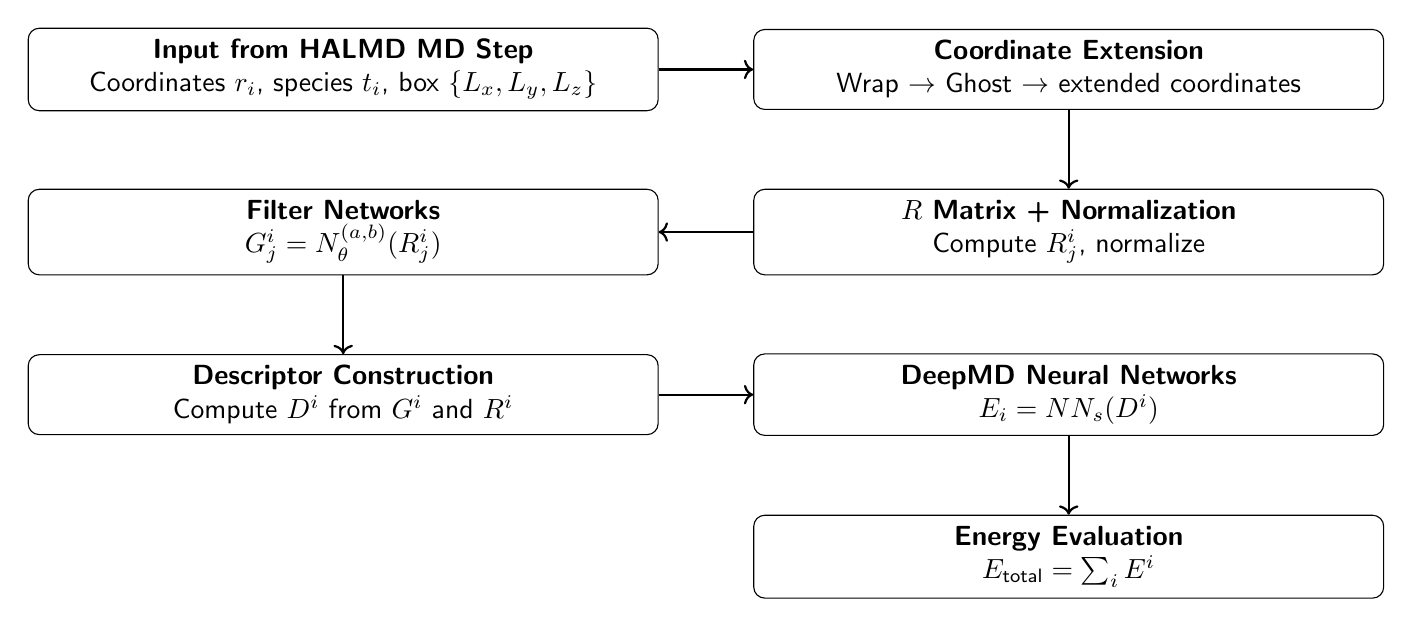
\begin{tikzpicture}[
    node distance=1.0cm and 1.2cm,
    box/.style={
        draw,
        rectangle,
        rounded corners,
        align=center,
        minimum width=8cm,
        minimum height=1.0cm,
        inner sep=4pt
    },
    arrow/.style={->, thick}
]

% Row 1
\node[box] (input) {%
\textbf{Input from HALMD MD Step}\\
Coordinates $r_i$, species $t_i$, box $\{L_x,L_y,L_z\}$
};

\node[box] (env) [right=of input] {%
\textbf{Coordinate Extension}\\
Wrap $\rightarrow$ Ghost $\rightarrow$ extended coordinates 
};

% Row 2
\node[box] (R) [below=of env] {%
\textbf{$R$ Matrix + Normalization}\\
Compute $R^i_{j}$, normalize
};

\node[box] (filter) [left=of R] {%
\textbf{Filter Networks}\\
$G^i_{j} =N_{\theta}^{(a,b)}(R^i_{j})$
};

% % Row 3
% \node[box] (G) [below=of filter] {%
% \textbf{$G$ Matrix Construction}\\
% Assemble $G_{ij}$
% };

\node[box] (D) [below=of filter] {%
\textbf{Descriptor Construction}\\
Compute $D^i$ from $G^i$ and $R^i$
};

% Row 4
\node[box] (nn) [right=of D] {%
\textbf{DeepMD Neural Networks}\\
$E_i = NN_s(D^i)$
};

\node[box] (energy) [below=of nn] {%
\textbf{Energy Evaluation}\\
$E_{\text{total}} = \sum_i E^i$
};



% Arrows
\draw[arrow] (input) -- (env);
\draw[arrow] (env) -- (R);
\draw[arrow] (R) -- (filter);
% \draw[arrow] (filter) -- (G);
\draw[arrow] (filter) -- (D);
\draw[arrow] (D) -- (nn);
\draw[arrow] (nn) -- (energy);


\end{tikzpicture}
\caption{DeepMD--HALMD energy evaluation pipeline implemented in this thesis.}
\end{figure}



\subsection{Model parameter extraction}
\label{sec:model_parameter_extraction}







\subsubsection{Frozen model structure}

The trained DeepMD-v2 potential is distributed as a frozen TensorFlow graph
(\texttt{frozen\_model.pb}).  
To perform manual inference inside HALMD, all relevant model parameters
must be reconstructed from the computation graph.  
The node list extracted from the model (see Appendix~X) contains all
information required for this reconstruction.

\paragraph{Descriptor attributes:}
The descriptor section of the graph exposes the physical and structural
parameters needed to build the environment matrix:
\begin{itemize}
    \item cutoff radii (\verb|descrpt_attr/rcut|, \verb|descrpt_attr/rcut_smth|),
    \item neighbour selection size (\verb|descrpt_attr/sel|, \verb|descrpt_attr/original_sel|),
    \item type mapping and normalization tensors  
          (\verb|descrpt_attr/t_avg|, \verb|descrpt_attr/t_std|, \verb|descrpt_attr/ntypes|).
\end{itemize}
These values uniquely determine the construction of $\hat{R}_i$ and ensure 
that HALMD reproduces the same geometric preprocessing as DeepMD.

\paragraph{Embedding network:}
The embedding (filter) network parameters appear under
\verb|filter_type_0/*|.  
The suffix \verb|_0| indicates that these parameters correspond to a central
atom of species \(a = 0\).  
DeepMD-v2 stores a separate filter (embedding) network for each central-atom
species, so in a multi-species system one would observe additional blocks such as
\verb|filter_type_1/*|, \verb|filter_type_2/*|, and so on.

Within each \verb|filter_type_a| group, DeepMD-v2 uses node names that follow the
pattern
\[
  \texttt{matrix\_}\ell\texttt{\_}b,
  \qquad
  \texttt{bias\_}\ell\texttt{\_}b,
\]
where:
\begin{itemize}
    \item $\ell$ is the layer index of the embedding MLP,
    \item $b$ is the \emph{neighbour-species index}.
\end{itemize}

Thus, nodes such as
\verb|matrix_1_0|, \verb|matrix_2_0|, \verb|matrix_3_0|
and their corresponding
\verb|bias_1_0|, \verb|bias_2_0|, \verb|bias_3_0|
represent the three-layer embedding network used when:
\[
\text{central species } a = 0, \qquad
\text{neighbour species } b = 0.
\]

In a multi-species model, additional blocks would appear, for example:
\begin{itemize}
    \item \verb|matrix_1_1|, \verb|matrix_2_1|, \dots  for neighbours of species \(b=1\),
    \item \verb|matrix_1_2|, \verb|matrix_2_2|, \dots  for neighbours of species \(b=2\), etc.
\end{itemize}

Each embedding layer provides:
\begin{itemize}
    \item a weight matrix (\texttt{matrix\_}$\ell$\texttt{\_}$b$),
    \item a bias vector (\texttt{bias\_}$\ell$\texttt{\_}$b$),
    \item a nonlinear activation function node (typically \verb|Tanh|).
\end{itemize}

Collectively, these nodes define the mapping

\begin{equation}
    \hat{s}_{ij} \mapsto G^i_{j}
\end{equation}


which transforms the normalized inverse distance into an embedding vector for
the descriptor.


\paragraph{Descriptor production:}
The node \verb|ProdEnvMatA| encapsulates the internal DeepMD operation that
produces the environment matrix and its derivatives:
\begin{itemize}
    \item relative positions and angular components (\verb|o_rmat|),
    \item pairwise distances (\verb|o_rij|),
    \item neighbour list (\verb|o_nlist|),
    \item geometric derivatives (\verb|o_rmat_deriv|).
\end{itemize}
These outputs provide the ground truth for validating HALMD's geometric
derivative implementation.

\paragraph{Fitting network:}
The atomic-energy fitting network appears under the node groups  
\verb|layer_0_type_0/*|, \verb|layer_1_type_0/*|,  
\verb|layer_2_type_0/*|, and \verb|final_layer_type_0/*|.  
Each layer contributes:
\begin{itemize}
    \item a weight matrix,
    \item a bias vector,
    \item optional residual-timestep coefficients (\verb|idt| nodes),
    \item a nonlinear activation function (\verb|Tanh|).
\end{itemize}
Together, these nodes define the mapping from the descriptor $D_i$ to the
atomic energy $E_i$.

\paragraph{Energy and force outputs.}
The frozen graph also includes nodes providing:
\begin{itemize}
    \item total energy (\verb|o_energy|),
    \item per-atom energy (\verb|o_atom_energy|),
    \item forces (\verb|o_force|),
    \item virials (\verb|o_virial|, \verb|o_atom_virial|),
\end{itemize}
as well as all intermediate gradient nodes under \verb|gradients/*|,
used by DeepMD's automatic differentiation engine.

\medskip
Together, these extracted components provide a complete specification of the
trained potential: descriptor parameters, embedding transformations,
environment-matrix construction, fitting-network architecture, and the final
energy/force outputs.  Using these elements, HALMD can reproduce DeepMD-v2
inference exactly, without relying on TensorFlow.


\subsubsection{Extraction procedure}

DeepMD-kit stores trained neural network potentials as a TensorFlow \texttt{frozen\_model.pb} file, accompanied by an \texttt{input.json} file containing model hyperparameters. The \texttt{.pb} file encodes all numerical weights, biases, and auxiliary tensors in the form of TensorFlow computation graph nodes, while the JSON file specifies the descriptor type, cutoff radius, number of neurons per layer, activation functions, and species layout. Following the methodology of DeepMD-kit v1 and v2 \cite{wang2018deepmd, zeng2023deepmdv2}, this thesis extracts all necessary model parameters from these files and converts them into an HDF5 representation suitable for efficient inference inside HALMD.

The extraction process begins by loading the TensorFlow graph definition from the \texttt{.pb} file. All tensors of type \texttt{Const} are scanned, and those whose node names match descriptor or fitting-network layers are decoded using TensorFlow’s low-level \texttt{tensor\_util.MakeNdarray}. The DeepMD model contains one set of parameters per atomic species, and the species ordering in the output strictly follows the ordering defined in the DeepMD input configuration. For the work presented here, the descriptor type is always the angular SE descriptor \texttt{se\_e2\_a}, which DeepMD-kit v2 uses for multi-species models requiring both radial and angular correlation encoding.

\paragraph{Descriptor parameters:}
For each species, the descriptor section consists of a stack of fully connected layers with user-specified neuron counts, activation functions, and optional residual time-step connections. The extraction script identifies each descriptor layer via a naming pattern of the form
% \[
% \texttt{filter\_type\_}<s>/\texttt{matrix\_}<k>_<t_n>, \qquad
% \texttt{filter\_type\_}<s>/\texttt{bias\_}<k>_{t_n},
% \]
\[
\mathtt{filter\_type\_}\langle s \rangle/\mathtt{matrix\_}\langle k \rangle\_\langle  t_n \rangle, \qquad
\mathtt{filter\_type\_}\langle s \rangle/\mathtt{bias\_}\langle k \rangle \_{\langle t_n \rangle},
\]
where \(s\) indexes the species, \(k\) is the layer index, and \(t_n\) enumerates neighbor-type channels. For each layer, the script records:
\begin{itemize}
    \item weight matrices,
    \item bias vectors,
    \item number of neurons,
    \item activation function (typically \texttt{tanh} or \texttt{linear} in the present work),
    \item the presence of a residual network branch.
\end{itemize}
DeepMD-v2 allows descriptor layers to use residual updates when \texttt{resnet\_dt=true}. In that case, a per-layer time-step tensor is extracted and marked in the output structure, though the use of residual updates depends on the model’s training configuration.

% \paragraph{Embedding (filter) network:}
% In the DeepMD architecture, the descriptor network is conceptually equivalent to the “filter” or embedding network described in \cite{wang2018deepmd, zeng2023deepmdv2}. Each species has its own filter-network parameters to account for species-dependent geometric correlations. The extracted filter-network weights are reshaped into a row-major layout compatible with HALMD’s GPU evaluation kernels.

\paragraph{Embedding (filter) network:}
In the DeepMD architecture, the descriptor network corresponds to the so-called filter or
embedding network \cite{wang2018deepmd,zeng2023deepmdv2}. This network transforms the
local geometric information of each neighbor—encoded through symmetry-preserving
descriptors—into a high-dimensional feature representation that captures many-body
correlations and chemical interactions. The embedding network consists of several fully
connected layers with nonlinear activation functions and is evaluated independently for
each neighbor atom.

Each atomic species is assigned its own set of embedding-network parameters, enabling
the model to represent species-dependent interaction patterns. The extracted filter-network
weights are reshaped into a row-major layout compatible with HALMD’s GPU evaluation
kernels.


\paragraph{Fitting network:}
For each species, the fitting network (also called the main network) predicts the atomic energy contribution \(E_i\). The extraction process retrieves:
\begin{itemize}
    \item all intermediate fitting layers,
    \item species-dependent activation functions,
    \item weight and bias tensors for each layer,
    \item the species-specific atomic energy bias term \texttt{bias\_atom\_e},
    \item the parameters of the final output layer.
\end{itemize}
The fitting-network layers are identified using a template of the form
\[
\texttt{layer\_LL\_type\_}<k>_<s>/\texttt{matrix}, \qquad 
\texttt{layer\_LL\_type\_}<k>_<s>/\texttt{bias},
\]
and similarly for the final layer \texttt{final\_layer\_type\_<s>}. The final layer uses a fixed activation function, typically \texttt{linear}, consistent with the DeepMD energy formulation.

\paragraph{Normalization parameters:}
DeepMD-v2 introduces descriptor normalization tensors \texttt{t\_avg} and \texttt{t\_std}, which are required to maintain numerical stability and descriptor smoothness. These tensors are extracted from the nodes
\[
\texttt{descrpt\_attr/t\_avg}, \qquad
\texttt{descrpt\_attr/t\_std},
\]
and stored in the HDF5 output so that HALMD can apply the same normalization as the original DeepMD model.

\paragraph{Organization and output format:}
All extracted parameters are written into a structured HDF5 file using a hierarchical layout:
\begin{itemize}
    \item global descriptor constants (cutoff radii, smoothing radii, normalization tensors),
    \item per-species descriptor network parameters,
    \item per-species fitting network parameters.
\end{itemize}
This structure mirrors the multi-species design of DeepMD-kit v2 and makes the extracted parameters directly usable by HALMD for inference. Unlike the single-species extraction used in the previous HALMD implementation \cite{cruz2025deepmd}, the present work extracts and stores fully species-resolved descriptor and fitting-network data, which are required for accurate multi-species DeepMD-v2 inference.

The resulting HDF5 file serves as the unified model representation for HALMD. During the simulation, HALMD loads this file, reconstructs the descriptor and neural networks using GPU-optimized data structures, and performs inference without relying on TensorFlow. This enables the deep potential model to be evaluated natively within HALMD’s simulation loop with high performance and full multi-species support.



\subsection{Coordinate system extension }
\label{sec:env_construction}

A roadmap for this section: we reconstruct the local atomic environment required by DeepMD-v2 through five stages—coordinate wrapping, ghost-cell generation, species-aware neighbour grouping, enforcement of the \texttt{sel} layout, and descriptor normalization—described in turn below.

A central contribution of this thesis is the redesign of HALMD’s environment–construction 
pipeline so that it follows the exact conventions required by DeepMD-v2. The earlier 
implementation by Cruz~\cite{cruz2025deepmd} relied on HALMD’s built-in periodic boundary 
handling and neighbour list, which correctly satisfy the minimum-image convention used in 
classical MD~\cite{colberg2011highly}. 
Under the minimum-image convention, the distance between two atoms is computed using only 
the closest periodic image of each particle, such that every interatomic separation lies 
within half the simulation box length in each Cartesian direction.

However, this approach provides only the minimal 
displacement between atoms and does not reproduce the full periodic environment expected by 
the DP descriptor pipeline. DeepMD-v2 requires explicit coordinate wrapping, 
ghost-cell expansion, species-aware neighbour grouping, and descriptor normalization 
\cite{wang2018deepmd, zeng2023deepmdv2}. These steps are essential for reproducing the 
descriptor inputs used during training.

The new DeePMD-style environment constructor introduced in this work consists of the following
components.

\subsubsection{Explicit coordinate wrapping}

DeepMD requires that all atomic coordinates are expressed inside the
primary simulation cell before any descriptor quantities are computed.
This is stricter than the minimum-image convention normally used in
classical molecular dynamics, where only the *differences* between
coordinates need to be mapped back into the simulation box.  
DeepMD, however, expects the \emph{absolute coordinates} of every atom to lie
within the interval $[0, L_\alpha)$ for each Cartesian direction
$\alpha \in \{x, y, z\}$.


To ensure consistency, each coordinate component is mapped explicitly
into the primary simulation box using
\begin{equation}
    \tilde{r}_{i\alpha}
    =
    r_{i\alpha}
    -
    L_\alpha 
    \left\lfloor \frac{r_{i\alpha}}{L_\alpha} \right\rfloor .
\end{equation}


This operation performs the following steps:

\begin{itemize}
    \item Compute the integer number of box lengths by which the particle
          has moved:
          \begin{equation}
            n_\alpha = \left\lfloor \frac{r_{i\alpha}}{L_\alpha} \right\rfloor .
          \end{equation}
         
          This may be positive (particle drifted to the right), negative
          (particle drifted to the left), or zero.

    \item Subtract exactly $n_\alpha L_\alpha$ from the coordinate so that
          the result lies in the interval $[0, L_\alpha)$:
          \begin{equation}
            \label{eq:coordinate_wrapping}
            \tilde{r}_{i\alpha} = r_{i\alpha} - n_\alpha L_\alpha 
          \end{equation}

    \item The wrapped coordinates $\tilde{\mathbf{r}}_i$ now correspond to
          the representation DeepMD expects as input.
\end{itemize}

This differs from the minimum-image convention, which only wraps
\emph{relative displacements}.  
DeepMD’s descriptor depends on absolute coordinates (through the
ghost-cell extension and species grouping), so the wrapping step is
necessary to guarantee that the computed descriptor matches the
TensorFlow implementation exactly.

% In summary, explicit coordinate wrapping enforces:

% \begin{itemize}
%     \item strict consistency with DeepMD-v2’s coordinate assumptions,
%     \item reproducible descriptor construction regardless of diffusion or
%           long simulation times,
%     \item the correct behaviour of ghost-cell expansion and neighbour
%           grouping.
% \end{itemize}

\subsubsection{Ghost-cell periodic extension}

DeepMD constructs atomic environments by explicitly replicating the simulation
cell in all spatial directions before evaluating descriptor quantities.  
This ensures that every atom, including those close to a periodic boundary,
retains a complete neighbourhood within the cutoff radius \( r_c \).  
In contrast, HALMD’s native neighbour list returns only the nearest periodic
image, which is sufficient for classical MD but does not supply the full set of
geometric relations required by the DeepMD descriptor pipeline.

To achieve DeepMD-compatible behaviour, the present work implements full
ghost-cell tiling. For each wrapped coordinate \( \tilde{\mathbf{r}}_i \), the
periodic images are generated as

\begin{equation}
\label{eq:ghost_expansion}
    \mathbf{r}_i^{(\mathbf{s})}
    =
    \tilde{\mathbf{r}}_i
    +
    s_x L_x\, \mathbf{e}_x
    +
    s_y L_y\, \mathbf{e}_y
    +
    s_z L_z\, \mathbf{e}_z,
    \qquad
    s_\alpha \in [-n_{\mathrm{buff},\alpha},\, n_{\mathrm{buff},\alpha}],
\end{equation}



where \(L_\alpha\) are the box lengths and 
\begin{equation}
    n_{\mathrm{buff},\alpha}
    =
    \Big\lceil \frac{r_c}{L_\alpha} \Big\rceil
\end{equation} 


ensures full spatial coverage of the cutoff sphere.  
For a cubic cell with \( n_{\mathrm{buff}} = 1 \), this produces
\(3^3 = 27\) images (the central box and its neighbouring tiles).  
Neighbour search is then performed over these images, and only the atoms whose
replicas fall within the cutoff are retained.

This explicit tiling is necessary for descriptor correctness: it guarantees that
all physically relevant neighbours are included, that the distances \( r_{ij} \)
and direction vectors \( \mathbf{r}_{ij} \) match those used by DeepMD-kit, and
that atoms near cell boundaries obtain descriptor rows identical to those of
atoms in the interior.  
By reproducing DeepMD's environment construction exactly, the HALMD
implementation achieves full compatibility with the DeepMD-v2 descriptor
generation process.





\subsubsection{Environment-matrix construction interface}
Previously, HALMD computed environment quantities directly from the neighbour list using 
minimum-image displacements.  
The new implementation builds environments from:
\begin{itemize}
    \item wrapped coordinates,
    \item ghost-expanded coordinates,
    \item species-ordered neighbour lists.
\end{itemize}
The construction of the descriptor matrices (\(R\), \(G\)) occurs later and is
documented in Section~3.4.

\subsubsection{Normalization using \texorpdfstring{\(t_{\mathrm{avg}}, t_{\mathrm{std}}\)}{tavg, tstd}}
DeepMD-v2 normalizes descriptor features using training-time statistics:
\[
\hat{X} = \frac{X - t_{\mathrm{avg}}}{t_{\mathrm{std}}}.
\]
The previous HALMD implementation lacked this step; the new pipeline integrates normalization 
directly, ensuring full compatibility with DeepMD-v2.

\subsubsection{Summary of improvements}
The updated environment-construction step introduces:
\begin{itemize}
    \item explicit DeePMD-style coordinate wrapping,
    \item full periodic ghost-cell expansion,
    \item species-aware neighbour grouping based on the \texttt{sel} configuration,
    \item a redesigned environment interface for descriptor construction,
    \item descriptor normalization matching DeepMD-v2.
\end{itemize}

These extensions form the necessary foundation for computing the \(R\) and \(G\) 
descriptor matrices (Section~3.4) and enable HALMD to accurately evaluate 
multi-species DeepMD-v2 models.


\subsubsection{Species-aware neighbour grouping}

DeepMD-v2 requires that neighbour atoms be organised in a very specific
species-dependent format before any descriptor quantities are computed.
This is fundamentally different from HALMD’s native neighbour list, which
treats all neighbours uniformly and returns a single distance-sorted list
independent of species.  
However, in DeepMD-v2 the descriptor is constructed under the assumption that
each central atom has a fixed, preallocated number of neighbour slots for 
\emph{each species type}, as defined by the model parameter \texttt{sel}:
\begin{equation}
    \texttt{sel} = 
    \bigl[
        N_c^{(1)},\,
        N_c^{(2)},\,
        \ldots,\,
        N_c^{(B)}
    \bigr]
    \label{eq:sel_vector}
\end{equation}

where $N_c^{(b)}$ is the number of neighbours of species $b$ that the model
expects for each central atom.

This fixed layout is not optional: every block of neighbours associated with a
neighbour species is passed through a species-specific embedding network
$N_{\theta}^{(a,b)}$, and thus the descriptor depends critically on 
\emph{which neighbour occupies which row} of the $R$ and $G$ matrices.

\paragraph{Constructing species-specific neighbour lists.}
To reproduce this behaviour, the new implementation replaces HALMD’s
species-blind neighbour structure with species-partitioned lists.
For a central atom $i$ and each species label $a$, HALMD now constructs
\[
\text{neighbors\_by\_type}[a]
=
\bigl\{\, j 
\;\big|\;
t_j = a,\; r_{ij} < r_c 
\,\bigr\},
\]
where $t_j$ is the species of neighbour $j$.
Each such list contains only the neighbours belonging to species $a$.



\paragraph{Sorting omitted for efficiency.}
In the reference DeepMD implementation, each species block of neighbours is
explicitly sorted by increasing interatomic distance,
\[
\text{neighbors\_by\_type}[a]
\;\leftarrow\;
\text{sort}\!\left(
\text{neighbors\_by\_type}[a],\; \text{key} = r_{ij}
\right),
\]
in order to impose a deterministic and easily interpretable layout of the
neighbour environments.  

In the present implementation, this explicit distance-based sorting step is
omitted. The subsequent construction of the environment matrices \(R\) and
\(G\), together with the associated embedding-network evaluation, preserves the
relative correspondence between neighbour entries and their geometric features.
Consequently, the numerical values of the resulting descriptors and predicted
energies remain invariant under permutations of neighbours within a given
species block.

Since the descriptor pipeline and fitting network are permutation-equivariant
within each species channel, removing the sorting step does not affect the
physical correctness of the model evaluation but eliminates an additional
\(\mathcal{O}(N \log N)\) cost per atom per species, thereby improving runtime
performance for large systems.


\subsubsection{Applying the \texttt{sel} constraint}

For each central atom, DeepMD-v2 requires that the descriptor contains a fixed
number of neighbour entries for each species, as prescribed by the vector
\(\texttt{sel}\) defined in Eq.~\eqref{eq:sel_vector}.
After grouping neighbours by species, each species block is adjusted to have
exactly \(N_c^{(a)}\) rows:
\[
\widehat{\mathrm{neighbors\_by\_type}}[a]
=
\begin{cases}
\text{first } N_c^{(a)} \text{ neighbours}, &
    \text{if more than } N_c^{(a)} \text{ are available}, \\[6pt]
\text{zero-padded rows}, &
    \text{if fewer than } N_c^{(a)} \text{ neighbours exist}.
\end{cases}
\]
This behaviour matches the DeepMD-v2 implementation, where missing neighbours
are represented by zero-valued geometric entries in the environment matrix resulting in
\[
R^i_{j} = [0, 0, 0, 0] 
% \hat{s}_{ij} = 0, \qquad
% G_{ij} = N^{(a,b)}_{\theta}(0),
\]
for all padded rows of environment matrices \(R\).

Zero-padding ensures that the assembled \(R\) matrices have the
fixed, model-dependent shape required by DeepMD-v2.



\paragraph{Constructing the full neighbour ordering.}
The final neighbour list for descriptor construction is obtained by concatenating
species blocks in the fixed species order used by the model:
\[
\text{neighbors\_ordered}
=
\bigl[
    \widehat{\text{neighbors\_by\_type}}[1],\;
    \widehat{\text{neighbors\_by\_type}}[2],\;
    \ldots,\;
    \widehat{\text{neighbors\_by\_type}}[B]
\bigr].
\]

Every descriptor row in the matrices $R$ and $G$ now corresponds to a specific
species and a specific position within that species block, exactly as expected
by the DeepMD-v2 architecture.

\paragraph{Importance of species grouping.}
This organisation is not merely a convenience; it is required because:
\begin{itemize}
    \item each species pair $(a,b)$ uses a different embedding network
          $N_{\theta}^{(a,b)}$,
    \item descriptor rows must map one-to-one to embedding-network evaluations,
    \item the quadratic descriptor $D_i$ implicitly assumes this grouping when
          computing $G^\mathrm{T}\hat{R}$,
    \item the fitting network is trained on descriptors in this exact ordering.
\end{itemize}

A deviation from this layout would result in incorrect $R$ and $G$ matrices,
leading to mismatched descriptors $D_i$, incorrect predicted energies, and
incorrect forces.

Thus, the introduction of species-aware neighbour grouping is a key requirement
for enabling HALMD to evaluate multi-species DeepMD-v2 models correctly.



\subsection{Construction of the configuration matrix \texorpdfstring{$R$}{R}}
\label{sec:R_matrix_construction}

This subsection derives the geometric configuration matrix \(R_i\) that serves as the direct input to the embedding network.

Once wrapped coordinates, ghost-cell expansions, and species-ordered neighbour
lists have been obtained (Section~\ref{sec:env_construction}), the next task is to
construct the geometric matrix $R^i$.  
This matrix encodes the local atomic environment of a central atom $i$ in a way that
is translationally, rotationally, and permutation invariant
\cite{wang2018deepmd,zeng2023deepmdv2}.  
Each of the $N_c^{\mathrm{(total)}}$ neighbour slots contributes one row of four geometric
quantities.

\subsubsection{Relative displacement}

Here, $\tilde{\mathbf r}_i$ denotes the wrapped coordinate of atom $i$ obtained by
the coordinate mapping in Eq.~\eqref{eq:coordinate_wrapping}, and
$\mathbf r_j^{(\mathbf s)}$ denotes the ghost-extended coordinate of neighbour
atom $j$ constructed via the periodic expansion in Eq.~\eqref{eq:ghost_expansion}.

The relative displacement vector and its magnitude are then given by
\begin{equation}\label{eq:relative_disp}
\mathbf r_{ij} = \mathbf r_j^{(\mathbf s)} - \tilde{\mathbf r}_i,
\qquad
r_{ij} = \lVert \mathbf r_{ij} \rVert .
\end{equation}

\subsubsection{Cutoff behaviour and switching function}

Following DeepMD, the radial switching function is defined as
\begin{equation}\label{eq:radial_switch}
s(r) =
\begin{cases}
\dfrac{1}{r}, & r < r_s, \\[6pt]
\dfrac{1}{r}\!\left[x^3(-6x^2 + 15x - 10) + 1\right], & r_s \le r < r_c, \\[10pt]
0, & r \ge r_c,
\end{cases}
\qquad
x = \dfrac{r - r_s}{r_c - r_s}.
\end{equation}

\subsubsection{Raw geometric matrix}

DeepMD defines the geometric features of neighbour $j$ of atom $i$ as
\begin{equation}
    (R^i)_j =
    \bigl[
        s(r_{ij}),\;
        s(r_{ij}) \dfrac{x_{ij}}{r_{ij}},\;
        s(r_{ij}) \dfrac{y_{ij}}{r_{ij}},\;
        s(r_{ij}) \dfrac{z_{ij}}{r_{ij}}
    \bigr]
    \in \mathbb R^{1 \times 4}.
\label{eq:raw_R_row}
\end{equation}

Collecting all neighbour rows yields the raw geometric matrix
\begin{equation}\label{eq:raw_geometric_matrix}
R^i \in \mathbb R^{N_c^{\mathrm{(total)}} \times 4}.
\end{equation}

\subsubsection{Species-aware neighbour ordering}

Neighbours are arranged by species and padded to fixed per-species capacities
prescribed by \texttt{sel} (Eq.~\eqref{eq:sel_vector}), yielding for every
atom a geometric matrix of identical shape, as described in Eq.~\eqref{eq:raw_geometric_matrix}.

\subsubsection{Feature normalization}

In the present implementation, the geometric matrix is further normalized using
training-time statistics
\[
t_{\mathrm{avg}}^i,\ t_{\mathrm{std}}^i \in \mathbb R^{N_c^{\mathrm{(total)}} \times 4}.
\]

The normalized matrix is defined as
\begin{equation}
\hat R^i_{k,\alpha}
=
\frac{R^i_{k,\alpha} - (t_{\mathrm{avg}}^i)_{k,\alpha}}
     {(t_{\mathrm{std}}^i)_{k,\alpha}},
\qquad
\hat R^i \in \mathbb R^{N_c^{\mathrm{(total)}} \times 4}.
\end{equation}

The first column
\[
\hat s_{ij} = \hat R^i_{j,0}
\]
serves as the scalar input to the embedding network.

\subsubsection{Summary}

The matrix $\hat R^i$ provides the complete geometric input for the subsequent
descriptor construction stage and is fully compatible with the DeepMD-v2
reference implementation.


\subsection{Construction of the embedding matrix \texorpdfstring{$G$}{G}}
\label{sec:G_matrix_construction}

Here we map the normalized inverse-distance features into learned embedding vectors \(G^i\) using the species-pair filter networks.

The second stage of the DeepPot-SE descriptor transforms each normalized inverse 
distance 
\[
\hat{s}_{ij} = \hat{R}^i_{j,0}
\]
into a high-dimensional embedding vector through a species-pair–specific 
\emph{filter network}.  
Collecting the embeddings for all neighbour slots produces the matrix
\[
G^i \in \mathbb{R}^{N_c^{\mathrm{(total)}} \times M},
\]
where $M$ is the embedding dimension and
$N_c^{\mathrm{(total)}} = \sum_b N_c^{(b)}$ is the total neighbour capacity specified by 
the model’s \texttt{sel} vector.

\subsubsection{Input and output dimensionality}

Each neighbour slot contributes a single scalar input
\[
\hat{s}_{ij} \in \mathbb{R},
\]
obtained from the first column of the normalized geometric matrix $\hat{R}^i$.

The embedding network maps this scalar to an $M$-dimensional output:
\[
G^i_{j:} \in \mathbb{R}^M.
\]

Stacking the embedding vectors for all neighbour rows yields
\[
G^i =
\begin{bmatrix}
(G^i_{1:})^{T} \\
(G^i_{2:})^{T} \\
\vdots \\
(G^i_{N_c^{(\mathrm{total})}:})^{T}
\end{bmatrix}
\in \mathbb{R}^{N_c^{\mathrm{(total)}} \times M}.
\]

The ordering of the rows is identical to the ordering of the rows of $\hat{R}^i$: 
neighbours are grouped by species and placed into fixed-capacity species blocks as prescribed by 
\texttt{sel}.

\subsubsection{Structure of the filter network}

For each central–neighbour species pair $(a,b)$, DeepMD-v2 defines a dedicated 
multi-layer perceptron (MLP)
\[
N^{(a,b)}_{\theta}: \mathbb{R} \to \mathbb{R}^M.
\]

Each of these MLPs consists of:
\begin{itemize}
    \item an input layer of width $1$ (the scalar $\hat{s}_{ij}$),
    \item $L$ hidden layers with species-pair–dependent widths,
    \item a final output layer of dimension $M$,
    \item Tanh activations between layers (except the output layer).
\end{itemize}

For a filter network with layer widths
\[
1 \;\to\; H_1 \;\to\; H_2 \;\to\; \cdots \;\to\; H_{L} \;\to\; M,
\]
the forward pass is
\begin{equation}
    \begin{aligned}
    h^{(1)} &= \tanh\!\left(W^{(1)}_{a,b}\,\hat{s}_{ij} + b^{(1)}_{a,b}\right), \\
    h^{(\ell)} &= \tanh\!\left(W^{(\ell)}_{a,b}\,h^{(\ell-1)} + b^{(\ell)}_{a,b}\right),
    \qquad \ell = 2,\dots,L, \\
    G^i_{j:} &= W^{(L+1)}_{a,b}\,h^{(L)} + b^{(L+1)}_{a,b}.
    \end{aligned} 
\end{equation}

These weights $W^{(\ell)}_{a,b}$ and biases $b^{(\ell)}_{a,b}$ are extracted from the frozen 
model under node names of the form  
\texttt{filter\_type\_a/matrix\_l\_b} and \texttt{filter\_type\_a/bias\_l\_b}.  
The subscript $b$ corresponds to the neighbour species, confirming explicitly that 
the network architecture depends on both the central and neighbour species.

\subsubsection{Species-pair dependent embedding networks}

For a central atom of species $a$ and a neighbour of species $b$, the embedding is 
computed using the matching filter network:
\[
G^i_{j:} = N^{(a,b(j))}_{\theta}\!\left( \hat{s}_{ij} \right).
\]

Different neighbour species therefore produce embeddings through different MLPs 
even when the geometric distances are identical.  
This mechanism is essential for modelling alloy systems, where cross-species interactions 
must be distinguishable in the descriptor.

HALMD stores the entire set of such networks in a two-dimensional structure:
\[
\texttt{neural\_networks}[a][b] \;\equiv\; N^{(a,b)}_{\theta}.
\]

\subsubsection{Runtime network selection and evaluation}

After species-grouped neighbour lists are constructed 
(Section~\ref{sec:env_construction}), each neighbour row $j$ is associated with a 
neighbour-species label $b(j)$.  
The embedding vector for that row is obtained via
\[
G^i_{j:} = N^{(a,b(j))}_{\theta}\!\left( \hat{s}_{ij} \right).
\]

The resulting $G^i_{j:}$ is stored in row $j$ of $G^i$.  
This ensures strict alignment between rows of $\hat{R}^i$ and rows of $G^i$, exactly as in the 
DeepMD-v2 computational graph.

\subsubsection{Summary}

The embedding matrix $G^i$ is constructed through the following steps:
\begin{itemize}
    \item extract the scalar geometric input $\hat{s}_{ij}$ from the normalized matrix $\hat{R}^i$,
    \item select the appropriate species-pair filter network $N^{(a,b)}_\theta$,
    \item evaluate its multi-layer structure using the trained weights and biases,
    \item assemble all embedding vectors into the matrix  
          $G^i \in \mathbb{R}^{N_c^{\mathrm{(total)}} \times M}$.
\end{itemize}

The resulting matrix provides the learned many-body representation that, together with 
$\hat{R}^i$, forms the complete input to the quadratic descriptor described in the next section.


\subsection{Descriptor Computation}
\label{sec:descriptor_computation}

The DeepPot-SE (\texttt{se\_e2\_a}) descriptor encodes the environment of a central atom \(i\)
through a combination of (i) normalized geometric features collected in the matrix
\(\hat{R}^i\) and (ii) learned nonlinear embeddings collected in the matrix \(G^i\).
These two matrices are then contracted into a quadratic descriptor \(D^i\), which forms the
input to the species-dependent fitting network predicting the atomic energy \(E^i\).

DeepMD-v2 assigns neighbour capacity on a per-species basis.  
Given species set \(\mathcal{S}\) and model parameters \(N_c^{(b)}\) for each species
\(b\in\mathcal{S}\), the total neighbour capacity is
\begin{equation}
   N_c^{\mathrm{(total)}} =
\sum_{b\in\mathcal{S}} N_c^{(b)} . 
\end{equation}

All matrices involved in descriptor computation are dimensioned using this total capacity.

% ------------------------------------------------------------
\subsubsection{Normalized geometric matrix}

Once the wrapped coordinates, periodic images, and species-ordered neighbour lists have been
constructed (Section~\ref{sec:env_construction}), the geometric features for atom \(i\) are
assembled into the matrix
\[
\hat{R}^i \in \mathbb{R}^{N_c^{\mathrm{(total)}} \times 4}.
\]

Each row corresponds to a specific neighbour slot and contains four quantities:
\begin{enumerate}
    \item the normalized inverse distance \(\hat{s}_{ij}\),
    \item the three normalized angular components
          \(\hat{x}_{ij}/r_{ij}^2\), \(\hat{y}_{ij}/r_{ij}^2\), \(\hat{z}_{ij}/r_{ij}^2\).
\end{enumerate}

Normalization follows the statistics extracted from the trained model:
\begin{equation}
    \hat{R}^i_{j,\alpha} =
    \frac{R_{ij,\alpha} - (t_{\mathrm{avg}})_{\alpha}}
        {(t_{\mathrm{std}})_{\alpha}},
    \qquad \alpha=0,\dots,3.
\end{equation}

The first column is used as the scalar geometric input for the nonlinear embedding:
\[
\hat{s}_{ij} = \hat{R}^i_{j,0}.
\]

This matrix therefore represents a geometrically structured, normalized description of the
neighbourhood of atom \(i\), with rows aligned to the species-block ordering of
DeepMD-v2.

% ------------------------------------------------------------
\subsubsection{Embedding matrix}

Each neighbour slot \(j\) has a known neighbour species \(b(j)\).  
DeepMD-v2 assigns a distinct filter (embedding) network for every central–neighbour pair
\((a,b)\), where \(a\) is the central species:
\[
G^i_{j:} = N_{\theta}^{(a,b(j))}(\hat{s}_{ij}),
\]
with \(N_{\theta}^{(a,b)} : \mathbb{R} \to \mathbb{R}^{M}\).

Evaluating all such networks yields
\[
G^i \in \mathbb{R}^{N_c^{\mathrm{(total)}} \times M}.
\]

Only the first \(M'\) embedding channels are required for the descriptor:
\begin{equation}
    G^{i,\mathrm{trunc}} = G^i[:,\,1:M'] \in
    \mathbb{R}^{N_c^{\mathrm{(total)}} \times M'}.   
\end{equation}

This embedding stage transforms the purely geometric scalar inputs \(\hat{s}_{ij}\) into
learned, species-dependent representations, with rows aligned exactly to the rows of
\(\hat{R}^i\).

% ------------------------------------------------------------
\subsubsection{Quadratic descriptor construction}

The DeepPot-SE descriptor is obtained by combining the geometric and embedding matrices into
a quadratic tensor:
\begin{equation}
    D^i
    =
    \frac{1}{(N_c^{\mathrm{(total)}})^2}
    \,
    \bigl((G^i)^\mathsf{T}\hat{R}^i\bigr)
    \bigl((\hat{R}^i)^\mathsf{T} G^{i,\mathrm{trunc}}\bigr).
\end{equation}

The intermediate products have the following shapes:
\[
\begin{aligned}
(G^i)^\mathsf{T}\hat{R}^i
&\in \mathbb{R}^{M \times 4},\\[4pt]
(\hat{R}^i)^\mathsf{T} G^{i,\mathrm{trunc}}
&\in \mathbb{R}^{4 \times M'},\\[4pt]
D^i &\in \mathbb{R}^{M \times M'}.
\end{aligned}
\]

DeepMD-v2 flattens this matrix in row-major order to obtain the final descriptor vector:
\[
\mathbf{D}^i \in \mathbb{R}^{M M'}.
\]

This vector is the complete learned representation of the neighbourhood of atom \(i\),
structured and normalized exactly as required by the DeepMD fitting network.

% ------------------------------------------------------------
\subsubsection{Summary}

The descriptor pipeline implemented in HALMD reproduces the DeepMD-v2 formulation without
modification. In particular:
\begin{itemize}
    \item the neighbour axis matches the species-resolved capacities \(N_c^{(b)}\),
    \item the geometric matrix \(\hat{R}^i\) implements all preprocessing steps required by
          DeepMD-v2,
    \item the embedding matrix \(G^i\) is produced by the full set of species-pair networks
          \(N_{\theta}^{(a,b)}\),
    \item the quadratic descriptor \(D^i\) and its scaling follow the DeepMD-v2 definition,
    \item the final descriptor vector \(\mathbf{D}^i\) matches TensorFlow output to
          floating-point precision.
\end{itemize}

This yields a complete, dimensionally consistent descriptor pipeline suitable for accurate,
high-performance DeepMD-v2 inference inside HALMD.


\subsection{Potential energy calculation}
\label{sec:potential_energy}

In the deep potential formalism, the total potential energy of a system of
\(N\) atoms is written as a sum of atomic contributions (Eq.~\eqref{eq:energy_decomp}),
where the atomic energy \(E^i\) is obtained by evaluating a \emph{species-dependent}
fitting neural network on the descriptor matrix \(\mathbf{D}^i\).
For an atom of species \(s_i\), the energy is computed as
\begin{equation}
    E^i = \mathrm{NN}_{s_i}(\mathbf{D}^i),
\end{equation}
where \(\mathrm{NN}_{s_i}\) denotes the DeepMD-v2 fitting network associated with
species \(s_i\).  
HALMD reconstructs these networks directly from the TensorFlow frozen graph
(\texttt{frozen\_model.pb}), including all linear layers, activation functions,
residual branches, and output transformations.

% ------------------------------------------------------------
\subsubsection{Baseline implementation prior to this Work}

The earlier HALMD implementation \cite{cruz2025deepmd} supported inference only for
\emph{single-species} DeepMD models.  
It successfully reproduced DeepMD energies for monoatomic systems but lacked the structural
components required for DeepMD-v2 multi-species inference:
\begin{itemize}
    \item only one fitting network for all atoms,
    \item no integration with multi-species descriptors (\(\hat{R}^i\), \(G^i\), \(D^i\)),
    \item no per-species energy shift (\texttt{bias\_atom\_e}),
    \item no mechanism for mapping descriptor matrices to the appropriate network.
\end{itemize}

Therefore, multi-component DeepMD-v2 models could not be evaluated within HALMD.

% ------------------------------------------------------------
\subsubsection{Species-dependent fitting networks}

DeepMD-v2 defines a separate fitting neural network for each atomic species.
In the TensorFlow graph, these networks appear under node groups of the form:
\[
\texttt{layer\_}\ell\texttt{\_type\_}a/\texttt{matrix}, \qquad
\texttt{layer\_}\ell\texttt{\_type\_}a/\texttt{bias}, \qquad
\texttt{final\_layer\_type\_}a/*,
\]
where:
\begin{itemize}
    \item \(a\) indexes the central-atom species,
    \item \(\ell\) is the layer index,
    \item each pair of \texttt{matrix} and \texttt{bias} nodes defines an affine layer.
\end{itemize}

HALMD reconstructs the complete set
\[
\bigl\{\,\mathrm{NN}_0,\ \mathrm{NN}_1,\ \dots,\ \mathrm{NN}_{S-1}\,\bigr\},
\]
and evaluates the appropriate network according to
\[
E^i = \mathrm{NN}_{s_i}(\mathbf{D}^i).
\]

The names of the corresponding TensorFlow nodes make the species mapping explicit:
\begin{itemize}
    \item for species \(a=0\):  
    \texttt{layer\_0\_type\_0/matrix},  
    \texttt{layer\_1\_type\_0/matrix},  
    \texttt{final\_layer\_type\_0/matrix}, etc.
    \item for species \(a=1\):  
    \texttt{layer\_0\_type\_1/matrix},  
    \texttt{layer\_1\_type\_1/matrix},  
    \texttt{final\_layer\_type\_1/matrix}, etc.
\end{itemize}

These node groups fully specify all weights and biases of each species-dependent fitting network.

% ------------------------------------------------------------
\subsubsection{Per-species energy offsets}

DeepMD-v2 optionally includes constant energy offsets for each species, stored under:
\[
\texttt{bias\_atom\_e}.
\]
HALMD extracts these tensors and evaluates
\begin{equation}
    E^i = \mathrm{NN}_{s_i}(\mathbf{D}^i) + b_{s_i}.
\end{equation}
This ensures that the final energy scale matches the one used during DeepMD model training.

% ------------------------------------------------------------
\subsubsection{Integration with the multi-species descriptor pipeline}

The descriptor matrix \(\mathbf{D}^i\) supplied to the fitting network has the exact structure
expected by the DeepMD-v2 TensorFlow implementation.  
Its construction incorporates:
\begin{itemize}
    \item the normalized geometric matrix  
    \(\hat{R}^i \in \mathbb{R}^{N_c^{\mathrm{(total)}} \times 4}\),
    \item neighbour-slot ordering based on the model's \texttt{sel} vector,
    \item embedding vectors from species-pair networks  
          \(N^{(a,b)}_\theta\!\left(\hat{s}_{ij}\right)\),
    \item truncation to the first \(M'\) embedding channels,
    \item the quadratic descriptor construction  
          \(D^i \in \mathbb{R}^{M \times M'}\),
    \item flattening into  
          \(\mathbf{D}^i \in \mathbb{R}^{MM'}\).
\end{itemize}

The ordering and dimensionality of \(\mathbf{D}^i\) must match the structure expected by
the fitting networks defined in  
\texttt{layer\_\*\_type\_a/*} and \texttt{final\_layer\_type\_a/*}.
The revised HALMD implementation enforces this consistency.

% ------------------------------------------------------------
\subsubsection{Reproduction of DeepMD-v2 energies}

With the full multi-species pipeline integrated, HALMD reproduces DeepMD-v2 energy predictions
to floating-point precision across all tested systems:
\begin{itemize}
    \item monoatomic models (Cu),
    \item multi-species alloy models (HEA),
    % \item oxide and ionic systems (garnet),
    \item alternative Copper models with different normalization statistics.
\end{itemize}

Both total energies and per-atom energies match DeepMD’s TensorFlow-based outputs.

% ------------------------------------------------------------
\subsubsection{Final formulation}

HALMD now evaluates the energy of each atom using the DeepMD-v2 expression
\begin{equation}
    E^i = \mathrm{NN}_{s_i}(\mathbf{D}^i) + b_{s_i},
\end{equation}
and accumulates the total energy as
\begin{equation}
    E_{\mathrm{tot}} = \sum_{i=1}^{N} E^i.
\end{equation}

This formulation is bitwise compatible with the DeepMD-v2 computational graph and is suitable
for high-performance molecular dynamics simulations of multi-species systems within HALMD.

\section{Force computation}
\label{sec:forces}

In the deep potential framework, forces are obtained as the negative 
gradient of the total potential energy with respect to atomic coordinates
as in Eq.~\eqref{eq:force_def}. 
Because the energy is produced through a multi-stage mapping involving geometric 
quantities (\(R\)), species-dependent embedding networks (\(G\)), and a 
species-dependent fitting network, the force computation requires evaluating a 
sequence of nested derivatives. 

DeepMD expresses this as a structured chain rule passing through:

\[
\mathbf{r}
\;\xrightarrow{\text{geometry}}\; 
R
\;\xrightarrow{\text{embedding}}\;
G
\;\xrightarrow{\text{fitting network}}\;
E,
\]
so that each force component involves contributions from all atoms appearing in 
the local environment of the corresponding descriptor.

The remainder of this section describes the derivative computation in HALMD.  
We begin with an overview of automatic differentiation (AD), which is used to 
evaluate all neural-network derivatives. We then detail the analytic derivatives 
of the geometry matrix \(R\), the descriptor \(D\), and finally show how these 
quantities are combined with the fitting-network derivatives to assemble the 
total atomic forces.


\subsection{Automatic Differentiation (AD)}
\label{sec:autodiff}

The computation of atomic forces in DeepMD requires propagating derivatives
through a sequence of transformations involving geometric preprocessing,
species-pair embedding networks, quadratic descriptor construction, and finally
a species-dependent fitting network.  
While the geometric derivatives admit closed-form expressions, the neural
networks involve nonlinear activations and residual connections that make
analytic differentiation impractical.  
For these components, HALMD employs \emph{automatic differentiation} (AD).

Automatic differentiation evaluates derivatives by decomposing a computation
into elementary operations and applying the chain rule locally
\cite{griewank2008evaluating,baydin2018automatic}.  
Two modes of AD are commonly used:

\subsubsection{Forward-mode AD (current HALMD implementation)}

Forward-mode AD propagates derivatives \emph{together with the value} of every
intermediate variable.  
Intuitively, each quantity in the computation carries a ``derivative tag’’ that
is updated whenever the variable participates in an operation.  

This mode is efficient when:
\begin{itemize}
    \item the number of inputs is small, and
    \item each function has a scalar or low-dimensional output.
\end{itemize}

These conditions hold for the DeepMD \emph{embedding networks}
$N_\theta^{(a,b)}$, each of which maps a single scalar input $\hat{s}_{ij}$ to
an $M$-dimensional output.  
HALMD therefore evaluates both the value
\[
G^i_{j}, \qquad \frac{\partial G^i_{j}}{\partial \hat{s}_{ij}}
\]
using forward-mode AD provided by Boost.Autodiff \cite{falcou2023boostautodiff}.

Forward-mode AD is also used in the fitting network to compute
$\partial E_i/\partial D_{i,\alpha}$, since each descriptor component
$D_{i,\alpha}$ can be marked as a differentiable input.

\subsubsection{Reverse-mode AD (not yet implemented)}

Reverse-mode AD performs the computation in two sweeps:
\begin{enumerate}
    \item a forward sweep computes all intermediate values,
    \item a backward sweep accumulates derivatives from the output back through
          the computational graph.
\end{enumerate}

Intuitively, reverse-mode AD works like backpropagation in neural networks:
one starts from the scalar loss (or, in this case, the atomic energy $E_i$)
and distributes sensitivities backward across all intermediate variables.

Reverse-mode AD is most efficient when:
\begin{itemize}
    \item the function has a \emph{single scalar output}, and
    \item the number of inputs is large.
\end{itemize}

This matches the structure of the \emph{fitting network}:
\[
E_i = \mathrm{NN}_{s_i}(\mathbf{D}^i),
\]
where the input dimension $\dim(\mathbf{D}_i) = MM'$ may be several hundred.
In such a setting, reverse-mode AD would greatly reduce computational cost, as
the full Jacobian $\partial E_i/\partial D_{i,\alpha}$ could be computed in a
\emph{single} backward pass.

At present, HALMD implements only forward-mode AD.  
Although correct, this results in one forward-mode evaluation per descriptor
entry, which is more expensive than necessary for large multi-species models.
Incorporating reverse-mode AD in the fitting network is therefore a
promising future improvement for performance-critical simulations.

\subsubsection{Hybrid analytic--AD differentiation}

All geometric derivatives---including those of the wrapped coordinates,
ghost-cell transformations, inverse-distance expressions, and switching
functions---are evaluated analytically.  
AD is used exclusively inside the neural-network components.  
This hybrid strategy offers:
\begin{itemize}
    \item exact agreement with the DeepMD-v2 TensorFlow implementation,
    \item efficient evaluation of nonlinear network derivatives,
    \item clear separation between analytic geometric contributions and AD-driven
          neural contributions.
\end{itemize}

The following sections detail the analytic components required to complete the
force calculation: derivatives of the geometric mapping, descriptor derivatives,
and the assembly of the total force.

\subsection{Derivatives of the Geometry Matrix \texorpdfstring{$R$}{R}}
\label{sec:R_derivative}

To compute forces, we require the derivative of each row of the geometry
matrix $R^{(i)}$ with respect to the coordinates of the central atom $i$.
Each row depends on the neighbour displacement defined in
Eq.~\eqref{eq:relative_disp}; we write
$\mathbf{r}_{ij} = (d_x, d_y, d_z)$ and $r_{ij} = \lVert \mathbf{r}_{ij} \rVert$,
and on the radial function
\[
s(r_{ij})
\]
defined in Section~\ref{sec:R_matrix_construction}.

We now derive all components of
\[
\frac{\partial R^{(i)}_{j\alpha}}{\partial \mathbf r_i}
\]
using only the multivariate chain rule.

% -------------------------------------------------------
\subsubsection{Step 1: Rewrite the Components of \texorpdfstring{$R$}{R}}

For neighbour $j$, we use the geometry row in Eq.~\eqref{eq:raw_R_row} with
the switched inverse distance $s(r_{ij})$ replaced by $\tilde{s}_{ij}$.

We denote the three directional components compactly as
\[
S_\alpha
=
\tilde{s}_{ij}\,\frac{d_\alpha}{r_{ij}},
\qquad
\alpha \in \{x,y,z\}.
\]

% -------------------------------------------------------
\subsubsection{Step 2: Derivative of the Distance \texorpdfstring{$r_{ij}$}{rij}}

Following the derivation in Section~\ref{sec:R_matrix_construction}, the
distance can be written as
\[
r_{ij} = (d_x^2 + d_y^2 + d_z^2)^{1/2}.
\]
Using the chain rule,
\[
\frac{\partial r_{ij}}{\partial d_\alpha}
=
\frac{d_\alpha}{r_{ij}},
\qquad
\alpha \in \{x,y,z\}.
\]
Since
\[
d_\alpha = r_{j,\alpha} - r_{i,\alpha},
\]
we also have
\[
\frac{\partial d_\alpha}{\partial \mathbf{r}_i}
= -\,\mathbf{e}_\alpha,
\]
and combining these yields
\[
\frac{\partial r_{ij}}{\partial \mathbf{r}_i}
=
\sum_\alpha
\frac{d_\alpha}{r_{ij}}(-\mathbf{e}_\alpha)
=
-\,\frac{1}{r_{ij}}(d_x, d_y, d_z)
=
-\,\hat{\mathbf{r}}_{ij}.
\]

% -------------------------------------------------------
\subsubsection{Step 3: Derivative of the Switching Function}

Using the switching function \(s(r)\) in Eq.~\eqref{eq:radial_switch}, define for
$r_s \le r < r_c$
\[
P(x) = x^3(-6x^2 + 15x - 10) + 1.
\]
Then
\[
\frac{dP}{dx} = x^2(-30x^2 + 60x - 30),
\qquad
\frac{dx}{dr} = \frac{1}{r_c - r_s}.
\]

The derivative of $s(r)$ is therefore
\begin{equation}
\frac{ds}{dr} =
\begin{cases}
-\dfrac{1}{r^2}, & r < r_s, \\[10pt]
-\dfrac{1}{r^2}P(x) + \dfrac{1}{r}\dfrac{dP}{dx}\dfrac{1}{r_c - r_s},
& r_s \le r < r_c, \\[12pt]
0, & r \ge r_c.
\end{cases}
\end{equation}

% -------------------------------------------------------


\subsubsection{Step 4: Derivative of the Radial Component}

The first component of the geometry row is
\[
R^{(i)}_{j0} = s(r_{ij}).
\]
Applying the chain rule,
\[
\frac{\partial R^{(i)}_{j0}}{\partial \mathbf r_i}
=
\frac{ds}{dr}(r_{ij})
\frac{\partial r_{ij}}{\partial \mathbf r_i}
=
-\,\frac{ds}{dr}(r_{ij})\,\hat{\mathbf r}_{ij}.
\]

% -------------------------------------------------------
\subsubsection{Step 5: Derivative of the Directional Components}

Each directional component is
\[
R^{(i)}_{j\alpha} = s(r_{ij})\,\frac{d_\alpha}{r_{ij}},
\qquad \alpha \in \{x,y,z\}.
\]

Using the product rule and the results of the previous steps,
\[
\frac{\partial R^{(i)}_{j\alpha}}{\partial \mathbf r_i}
=
-\,\frac{ds}{dr}(r_{ij})\frac{d_\alpha}{r_{ij}}\,\hat{\mathbf r}_{ij}
- s(r_{ij})\,\frac{1}{r_{ij}}\mathbf e_\alpha
+ s(r_{ij})\,\frac{d_\alpha}{r_{ij}^2}\,\hat{\mathbf r}_{ij}.
\]

This formula provides the complete derivative of the directional components
$R^{(i)}_{j1}, R^{(i)}_{j2}, R^{(i)}_{j3}$.

% -------------------------------------------------------
\subsubsection{Step 6: Normalized Geometry Derivative}

Note that the raw radial feature $s(r_{ij}) = R^{(i)}_{j0}$ becomes the normalized
quantity $\hat s_{ij} := \hat R^{(i)}_{j0}$ after feature normalization, and it is
this normalized scalar $\hat s_{ij}$ that is used as the input to the embedding
network.

DeepMD-v2 uses component-wise normalization:
\[
\hat R^{(i)}_{j\alpha}
=
\frac{
    R^{(i)}_{j\alpha} - (t_{\mathrm{avg}})_\alpha
}{
    (t_{\mathrm{std}})_\alpha
}.
\]
Since the normalization parameters are constants,
\begin{equation}
   \frac{\partial \hat R^{(i)}_{j\alpha}}{\partial \mathbf{r}_i}
    =
    \frac{1}{(t_{\mathrm{std}})_\alpha}
    \frac{\partial R^{(i)}_{j\alpha}}{\partial \mathbf{r}_i}. 
\end{equation}

% -------------------------------------------------------
\subsubsection{Step 7: Derivative with Respect to the Neighbour Coordinate \texorpdfstring{$\mathbf{r}_j$}{rj}}

All formulas above were derived for the derivative with respect to the
\emph{central} atom $i$.  
The derivative with respect to the \emph{neighbour} atom $j$ is obtained
immediately from the identity
\[
\mathbf{r}_{ij} = \mathbf{r}_j - \mathbf{r}_i,
\]
which implies
\[
\frac{\partial d_\alpha}{\partial \mathbf{r}_j}
= +\,\mathbf{e}_\alpha,
\qquad
\text{and}
\qquad
\frac{\partial d_\alpha}{\partial \mathbf{r}_i}
= -\,\mathbf{e}_\alpha.
\]

Using the chain rule for the distance $r_{ij}$,
\begin{equation}
    \frac{\partial r_{ij}}{\partial \mathbf{r}_j}
    =
    \sum_\alpha
    \frac{\partial r_{ij}}{\partial d_\alpha}
    \frac{\partial d_\alpha}{\partial \mathbf{r}_j}
    =
    \sum_\alpha
    \frac{d_\alpha}{r_{ij}}\,\mathbf{e}_\alpha
    =
    +\,\hat{\mathbf{r}}_{ij},
\end{equation}

which is exactly the opposite of the central-atom derivative
$\partial r_{ij}/\partial \mathbf{r}_i = -\hat{\mathbf{r}}_{ij}$.

\vspace{1em}

\noindent\textit{As a consequence, every derivative with respect to}
$\mathbf{r}_j$
\textit{is simply the negative of the corresponding derivative with respect to}
$\mathbf{r}_i$:
\[
\frac{\partial R^{(i)}_{j\alpha}}{\partial \mathbf{r}_j}
=
-\,
\frac{\partial R^{(i)}_{j\alpha}}{\partial \mathbf{r}_i},
\qquad
\alpha = 0,1,2,3.
\]

This follows because every dependence of $R^{(i)}_{j\alpha}$ on atomic positions
appears only through the displacement vector $\mathbf{r}_{ij}$, and exchanging the
differentiation variable from $\mathbf{r}_i$ to $\mathbf{r}_j$ reverses the
sign of every chain-rule factor:
\[
\frac{\partial}{\partial \mathbf{r}_j}
(\mathbf{r}_j - \mathbf{r}_i)
= +\mathbf{I},
\qquad
\frac{\partial}{\partial \mathbf{r}_i}
(\mathbf{r}_j - \mathbf{r}_i)
= -\mathbf{I}.
\]

Thus, once the derivative with respect to the central atom is known, the
neighbour-atom derivative requires no further computation.


\subsection{Derivative of the Embedding Matrix}
\label{sec:G_derivative}

For each central atom $i$, the embedding matrix
\[
G^{(i)} \in \mathbb{R}^{N_c \times M}
\]
is produced by species-dependent embedding networks applied to the local
environment of atom $i$.  
Each row depends on the local geometry only through the scalar input
\[
\hat s_{ij} := \hat R^{(i)}_{j0},
\]
the first (radial) component of the normalized geometric matrix.

Hence, for each neighbour $j$,
\[
G^{(i)}_{j:} = \mathrm{N}^{(a,b)}_{\theta}\!\left(\hat s_{ij}\right).
\]

The derivative of $G^{(i)}$ with respect to the geometry therefore reduces to the
one–dimensional derivative of the embedding network with respect to its scalar
input:
\begin{equation}
\boxed{
\frac{\partial G^{(i)}_{jp}}{\partial \hat R^{(i)}_{j0}}
=
\frac{d\,\mathrm{N}^{(a,b)}_{\theta,p}}{d \hat s}\!\left(\hat s_{ij}\right),
\qquad
p = 1,\dots,M.
}
\end{equation}

All other components of $\hat R^{(i)}$ do not influence $G^{(i)}$:
\[
\frac{\partial G^{(i)}_{jp}}{\partial \hat R^{(i)}_{j\alpha}} = 0,
\qquad \alpha \neq 0.
\]

The vector
\[
\mathbf q^{(i)}_j :=
\left(
\frac{\partial G^{(i)}_{j1}}{\partial \hat R^{(i)}_{j0}},
\ldots,
\frac{\partial G^{(i)}_{jM}}{\partial \hat R^{(i)}_{j0}}
\right)
\in \mathbb{R}^M
\]
is obtained by automatic differentiation of the embedding network and is treated
as a known quantity in the subsequent descriptor and force derivations.


\subsection{Descriptor Derivative}
\label{sec:descriptor_derivative}

For each central atom $i$, the DeepPot-SE descriptor is constructed from the
interaction between the embedding matrix
$G^{(i)} \in \mathbb{R}^{N_c \times M}$
and the normalized geometric matrix
$\hat R^{(i)} \in \mathbb{R}^{N_c \times 4}$.
Their contraction enters through the intermediate matrix
\[
C^{(i)} = \frac{1}{N_c} \big(G^{(i)}\big)^{\mathsf T} \hat R^{(i)},
\qquad
C^{(i)} \in \mathbb{R}^{M \times 4}.
\]
The matrix $C^{(i)}$ aggregates all geometry–embedding interactions and forms the
foundation of the quadratic descriptor used in DeepMD.

\medskip

The full (extended) descriptor is defined as the Gram matrix
\begin{equation}
    D^{(i)}_{\mathrm{ext}}
    =
    C^{(i)} \big(C^{(i)}\big)^{\mathsf T},
    \qquad
    D^{(i)}_{\mathrm{ext}} \in \mathbb{R}^{M \times M}.
\end{equation}

This construction ensures permutation invariance of neighbours and couples all
embedding channels quadratically.

However, the actual DeepPot-SE descriptor used by the fitting network consists
only of the first $M'$ columns of $D^{(i)}_{\mathrm{ext}}$:
\begin{equation}
    D^{(i)} = D^{(i)}_{\mathrm{ext}}\,P,
    \qquad
    D^{(i)} \in \mathbb{R}^{M \times M'}.
\end{equation}

Here \(P \in \mathbb{R}^{M \times M'}\) is the column-selection matrix
\[
P =
\begin{bmatrix}
I_{M'} \\
0_{(M - M') \times M'}
\end{bmatrix},
\]
so that multiplication by \(P\) is equivalent to retaining the first \(M'\) columns of \(D^{(i)}_{\mathrm{ext}}\).

Thus, the descriptor truncation is implemented by a simple column restriction.

\subsubsection*{Derivative with respect to the intermediate matrix $C^{(i)}$}

From the component definition
\[
\big(D^{(i)}_{\mathrm{ext}}\big)_{mn}
=
\sum_{\alpha=1}^{4} C^{(i)}_{m\alpha} C^{(i)}_{n\alpha},
\]
the derivative of $D^{(i)}_{\mathrm{ext}}$ with respect to one entry
$C^{(i)}_{p\beta}$ follows by direct application of the product rule:
\[
\frac{\partial \big(D^{(i)}_{\mathrm{ext}}\big)_{mn}}
     {\partial C^{(i)}_{p\beta}}
=
\delta_{mp} C^{(i)}_{n\beta}
+
\delta_{np} C^{(i)}_{m\beta},
\]
where $\delta_{ij}$ denotes the Kronecker delta.

Since the network descriptor $D^{(i)}$ retains only the first $M'$ columns of
$D^{(i)}_{\mathrm{ext}}$, the corresponding derivative is
\[
\frac{\partial D^{(i)}_{mn}}{\partial C^{(i)}_{p\beta}}
=
\delta_{mp} C^{(i)}_{n\beta}
+
\delta_{np} C^{(i)}_{m\beta},
\qquad n \le M'.
\]

\subsubsection*{Derivative with respect to the normalized geometric matrix}

The intermediate matrix
\[
C^{(i)} = \frac{1}{N_c} \big(G^{(i)}\big)^{\mathsf T} \hat R^{(i)}
\]
depends on $\hat R^{(i)}$ in two distinct ways:
(i) explicitly through the right factor $\hat R^{(i)}$, and
(ii) implicitly through the embedding matrix $G^{(i)}$, since each row
$G^{(i)}_{j:}$ is produced by the embedding network from the scalar input
\[
\hat s_{ij} := \hat R^{(i)}_{j0}.
\]

Accordingly, the derivative of $C^{(i)}$ with respect to $\hat R^{(i)}$ must be
decomposed into an explicit and an implicit contribution,
\[
\frac{\partial C^{(i)}}{\partial \hat R^{(i)}}
=
\left.\frac{\partial C^{(i)}}{\partial \hat R^{(i)}}\right|_{G}
+
\left.\frac{\partial C^{(i)}}{\partial G^{(i)}}\right|_{\hat R}
\frac{\partial G^{(i)}}{\partial \hat R^{(i)}}.
\]

In component form, using
\[
C^{(i)}_{p\beta} = \frac{1}{N_c} \sum_{j=1}^{N_c} G^{(i)}_{jp} \hat R^{(i)}_{j\beta},
\]
the explicit contribution is
\[
\left.\frac{\partial C^{(i)}_{p\beta}}{\partial \hat R^{(i)}_{j\alpha}}\right|_{G}
=
\frac{1}{N_c} G^{(i)}_{jp} \delta_{\beta\alpha}.
\]

Since the embedding matrix $G^{(i)}$ depends on $\hat R^{(i)}$ only through
$\hat R^{(i)}_{j0}$, the implicit contribution is
\[
\frac{\partial G^{(i)}_{\ell p}}{\partial \hat R^{(i)}_{j\alpha}}
=
\delta_{\ell j}\,\delta_{0\alpha}
\frac{\partial G^{(i)}_{jp}}{\partial \hat R^{(i)}_{j0}}.
\]

Substituting yields the full derivative
\[
\boxed{
\frac{\partial C^{(i)}_{p\beta}}{\partial \hat R^{(i)}_{j\alpha}}
=
\frac{1}{N_c} G^{(i)}_{jp} \delta_{\beta\alpha}
+
\frac{1}{N_c} \delta_{0\alpha}
\frac{\partial G^{(i)}_{jp}}{\partial \hat R^{(i)}_{j0}}
\hat R^{(i)}_{j\beta}.
}
\]

\medskip
\noindent\textbf{Descriptor derivative with respect to $\hat R^{(i)}$.}
For $n \le M'$,
\[
\boxed{
\frac{\partial D^{(i)}_{mn}}{\partial \hat R^{(i)}_{j\alpha}}
=
\frac{1}{N_c}
\big( G^{(i)}_{jm} C^{(i)}_{n\alpha} + G^{(i)}_{jn} C^{(i)}_{m\alpha} \big)
+
\frac{1}{N_c} \delta_{0\alpha}
\left(
\frac{\partial G^{(i)}_{jm}}{\partial \hat R^{(i)}_{j0}}
\sum_{\beta} \hat R^{(i)}_{j\beta} C^{(i)}_{n\beta}
+
\frac{\partial G^{(i)}_{jn}}{\partial \hat R^{(i)}_{j0}}
\sum_{\beta} \hat R^{(i)}_{j\beta} C^{(i)}_{m\beta}
\right).
}
\]

This expression shows explicitly that only the radial component
$\hat R^{(i)}_{j0}$ influences the descriptor through the embedding network,
while the remaining geometric components affect $C^{(i)}$ only through the
direct linear term.




\subsection{Fitting Network Derivative}
\label{sec:fitting_network_derivative}

Here we differentiate the species-dependent fitting networks so that descriptor sensitivities yield atomic-energy gradients.

The final stage of the DeepMD--v2 force pipeline is the differentiation of the
species-dependent fitting network that maps the descriptor of atom~$i$ to its atomic
energy,
\[
E^i = \mathrm{NN}_{s_i}\!\bigl(\mathrm{vec}(D^i)\bigr),
\]
where $s_i$ denotes the species of atom~$i$ and
\[
D^i \in \mathbb{R}^{M \times M'}
\]
is the (truncated) descriptor matrix constructed in
Section~\ref{sec:descriptor_computation}.  
The fitting network consumes the flattened descriptor
$\mathrm{vec}(D^i) \in \mathbb{R}^{MM'}$.

To assemble forces, we require the Jacobian of $E^i$ with respect to the full
descriptor matrix:
\begin{equation}
\boxed{
J^i
:=
\frac{\partial E^i}{\partial D^i}
\in \mathbb{R}^{M \times M'},
\qquad
(J^i)_{mn} = \frac{\partial E^i}{\partial D^i_{mn}}.
}
\end{equation}

In the frozen TensorFlow graph, the fitting network for species $s$ is encoded by
nodes such as
\[
\begin{aligned}
\texttt{layer\_0\_type\_s/matrix},\quad
\texttt{layer\_0\_type\_s/bias}, \\
\dots,\quad
\texttt{final\_layer\_type\_s/matrix},\quad
\texttt{final\_layer\_type\_s/bias}.
\end{aligned}
\]
together with optional residual-scaling nodes \texttt{idt} and the per-species energy
offset \texttt{bias\_atom\_e}.  
These parameters are extracted as described in
Section~\ref{sec:model_parameter_extraction} and reconstructed in HALMD’s
neural-network module.

\subsubsection{Forward-mode automatic differentiation of the fitting network}

The fitting networks in DeepMD--v2 consist of several fully connected layers with
nonlinear activation functions, optional residual connections, and timestep-related
scalings.  
The resulting mapping
\[
\mathrm{vec}(D^i) \longmapsto E^i
\]
is highly nonlinear, and an explicit hand-derived expression for
$\partial E^i / \partial D^i_{mn}$ would be lengthy and error-prone.

Instead, HALMD evaluates these derivatives using \emph{forward-mode automatic
differentiation} (AD) provided by Boost.Autodiff~\cite{falcou2023boostautodiff}.  
Conceptually, forward-mode AD augments each input component with an ``infinitesimal''
tangent and propagates both value and derivative through all primitive operations.

For the fitting network, this proceeds as follows for each flattened descriptor
index $\alpha \in \{1,\dotsc,MM'\}$:

\begin{enumerate}
    \item The descriptor matrix $D^i$ is flattened to $\mathrm{vec}(D^i)$ and
          promoted to an array of autodiff variables. The $\alpha$-th component is
          seeded with unit tangent and all others with zero tangent.

    \item This augmented input is propagated forward through all layers of the
          network, using the same weights, biases, activation functions, and
          residual connections as in the standard inference.

    \item At the output, the autodiff scalar representing $E^i$ contains both the
          energy value and its derivative with respect to
          $\mathrm{vec}(D^i)_\alpha$.  
          The derivative part is read out as
          $\partial E^i / \partial \mathrm{vec}(D^i)_\alpha$.
\end{enumerate}

Repeating this procedure for $\alpha = 1,\dotsc,MM'$ yields the full gradient with
respect to the flattened descriptor,
\[
\frac{\partial E^i}{\partial \mathrm{vec}(D^i)} \in \mathbb{R}^{MM'}.
\]
Reshaping this vector back to matrix form gives the Jacobian
\begin{equation}
\boxed{
J^i
=
\mathrm{reshape}_{M\times M'}\!\left(
\frac{\partial E^i}{\partial \mathrm{vec}(D^i)}
\right)
\in \mathbb{R}^{M\times M'}.
}
\end{equation}

From an algorithmic point of view, this is equivalent to computing one forward
pass per descriptor entry, i.e.\ the cost scales linearly with $MM'$.  
For the descriptor sizes considered in this work, this is acceptable and greatly
simplifies the implementation because no explicit backpropagation code is required.

\subsubsection{Relation to reverse-mode AD and future improvements}

For scalar outputs and high-dimensional inputs, \emph{reverse-mode} AD is
theoretically more efficient than forward mode, as it computes the entire gradient
$\partial E^i / \partial \mathrm{vec}(D^i)$ in a single backward sweep.  
This is the strategy employed by deep-learning frameworks such as
TensorFlow~\cite{abadi2016tensorflow} and PyTorch~\cite{paszke2019pytorch}.

In the present HALMD implementation, only forward-mode AD has been realized for the
fitting networks.  
Extending the neural-network module to support reverse-mode AD would reduce the
asymptotic cost of gradient evaluation and is therefore a natural target for future
optimisation.  
Nevertheless, the forward-mode approach used here already provides exact
derivatives of the reconstructed fitting networks and is sufficient to achieve
bitwise agreement with DeepMD--v2 energies and forces for all tested models.



\subsection{Final Force Assembly}
\label{sec:final_force_assembly}

We now assemble all derivative components derived in the preceding sections to
obtain the explicit DeepMD--v2 force expression. Starting from the energy
decomposition in Eq.~\eqref{eq:energy_decomp}, the force on atom $k$ is

\begin{equation}
\mathbf{F}_k
=
-\,\frac{\partial E}{\partial \mathbf{r}_k}
=
-\,\sum_{i}
\frac{\partial E^i}{\partial \mathbf{r}_k}.
\end{equation}

Using the chain rule along the descriptor construction pathway
\[
\mathbf{r}
\;\longrightarrow\;
\hat{R}^i
\;\longrightarrow\;
G^i
\;\longrightarrow\;
C^i
\;\longrightarrow\;
D^i
\;\longrightarrow\;
E^i,
\]
we obtain
\begin{equation}
\boxed{
\mathbf{F}_k
=
-
\sum_i
\sum_{m=1}^{M} \sum_{n=1}^{M'}
J^i_{mn}
\,
\frac{\partial D^i_{mn}}{\partial \mathbf{r}_k}
}
\end{equation}
where
\begin{equation}
\boxed{
J^i := \frac{\partial E^i}{\partial D^i} \in \mathbb{R}^{M \times M'}.
}
\end{equation}

% ---------------------------------------------------------

\subsubsection{Descriptor--level contribution}

From Section~\ref{sec:descriptor_derivative}, the derivative of the descriptor
with respect to the normalized geometry is
\begin{equation}
\boxed{
\frac{\partial D^i_{mn}}{\partial \hat R^i_{j\alpha}}
=
\frac{1}{N_c}
\left(
G^i_{jm} C^i_{n\alpha} + G^i_{jn} C^i_{m\alpha}
\right)
+
\frac{1}{N_c}\,\delta_{0\alpha}
\left(
\frac{\partial G^i_{jm}}{\partial \hat R^i_{j0}}
\sum_{\beta} \hat R^i_{j\beta} C^i_{n\beta}
+
\frac{\partial G^i_{jn}}{\partial \hat R^i_{j0}}
\sum_{\beta} \hat R^i_{j\beta} C^i_{m\beta}
\right).
}
\end{equation}

% ---------------------------------------------------------

\subsubsection{Geometric contribution}

The normalized geometry depends explicitly on the atomic coordinates, and its
analytic derivative
\[
\frac{\partial \hat R^i_{j\alpha}}{\partial \mathbf r_k}
\]
was derived in Section~\ref{sec:R_derivative}. This term contains the complete
geometric information (relative displacements, inverse distances, directional
components, and switching functions).

% ---------------------------------------------------------

\subsubsection{Final force expression}

Combining the descriptor derivative with the geometric derivative yields the
explicit DeepMD--v2 force:

\begin{equation}
\boxed{
\mathbf F_k
=
-
\sum_i
\sum_j
\sum_{m=1}^{M} \sum_{n=1}^{M'}
J^i_{mn}
\,
\frac{\partial D^i_{mn}}{\partial \hat R^i_{j\alpha}}
\,
\frac{\partial \hat R^i_{j\alpha}}{\partial \mathbf r_k}.
}
\end{equation}

This expression decomposes the force into a purely neural contribution
(\(J^i\) and \(\partial G^i / \partial \hat R^i_{j0}\)) and an analytic geometric
contribution (\(\partial \hat R^i / \partial \mathbf r_k\)), making the entire
force evaluation mathematically explicit and numerically stable.

\medskip

Equation~\eqref{sec:final_force_assembly} therefore reconstructs the full
DeepMD--v2 force pathway in HALMD using a consistent hybrid of analytic geometry
and automatic differentiation for the neural components.



\section{Results}
\label{sec:results}

This chapter presents the numerical results obtained from the HALMD
implementation of the DeepMD-v2 descriptor, fitting network, and force
derivatives developed in this thesis.
The primary goal of the evaluation is to verify that HALMD reproduces the
reference DeepMD-v2 behaviour for energies and, as far as possible, for force
derivatives.  
Because the force pipeline is significantly more complex and highly sensitive
to the analytical--AD derivative chain, special emphasis is placed on
identifying where agreement is achieved and where discrepancies remain.

\vspace{0.5em}

The tests were conducted using several trained DeepMD-v2 models:

\begin{itemize}
    \item a monoatomic Cu model (Model A),
    \item a multi-component high-entropy alloy model (HEA),
    \item a garnet model,
    \item a second Cu model (Model B), trained on a different dataset and
          exhibiting noticeably different tensor statistics.
\end{itemize}


% ===========================================================
\subsection{Energy agreement between DeepMD and HALMD}

A key requirement for correctness is the reproduction of per-atom and total
energies predicted by DeepMD.
Because the HALMD implementation now includes the full descriptor,
species-dependent filter networks, fitting networks, and bias terms,
the predicted energies should match DeepMD up to floating-point precision.

A practical consideration in this comparison is numerical precision.
DeepMD reference energies are evaluated in double precision within the
TensorFlow framework, whereas the HALMD implementation evaluates the
DeepMD-v2 inference pipeline primarily in single-precision floating-point
arithmetic on the GPU for performance reasons.
For this reason, agreement is assessed at the level of single-precision
floating-point accuracy, and HALMD energies are reported accordingly.

Tables~\ref{tab:energy-cu}--\ref{tab:energy-garnet} illustrate this agreement
for several trained models.

% -----------------------------------------------------------
\subsubsection*{Monoatomic Copper model (model A)\cite{Cu_fcc_slabs_2023}}

\begin{table}[H]
\centering
\caption{Energy comparison for the Cu model.
HALMD energies are evaluated in single precision; DeepMD energies are shown
as produced by the reference implementation.}
\label{tab:energy-cu}
\begin{tabular}{cccc}
\hline
Cells & Atoms & DeepMD Energy (eV) & HALMD Energy (eV) \\
\hline
$1\times1\times1$ & 4   & $-6673.84$ & $-6673.84$ \\
$2\times2\times2$ & 32   & $-53412.4$ & $-53412.4$ \\
$3\times3\times3$ & 108   & $-180303$ & $-180303$ \\
$4\times4\times4$ & 256   & $-427425$ & $-427425$ \\
\hline
\end{tabular}
\end{table}

Agreement is exact up to single-precision floating-point accuracy, with
remaining differences attributable to rounding.

% -----------------------------------------------------------

\subsubsection*{High-entropy alloy (HEA) model \cite{deepmdkit_v2_data}}

\begin{table}[H]
\centering
\caption{Energy comparison for the HEA model.
HALMD energies are evaluated in single-precision arithmetic on the GPU.}
\label{tab:energy-hea}
\begin{tabular}{cccc}
\hline
Cells & Atoms & DeepMD Energy (eV) & HALMD Energy (eV) \\
\hline
$1\times1\times1$ & 16   & $-66.7551048$ & $-66.7551$ \\
$2\times2\times2$ & 128   & $-895.49828775$ & $-895.498$ \\
$3\times3\times3$ & 432   & $-3490.86044623$ & $-3490.86$ \\
% $4\times4\times4$ & 1024   & $-10677.90008914$ & $-XXXXXX.XXXX$ \\
\hline
\end{tabular}
\end{table}

Agreement is exact up to single-precision floating-point accuracy across
all tested system sizes.

% -----------------------------------------------------------

\subsubsection*{Garnet model \cite{zhong2025hydrogen}}

\begin{table}[H]
\centering
\caption{Energy comparison for the garnet model used in
\cite{zhong2025hydrogen} using the same configuration used in the paper. HALMD energies are reported at single-precision
accuracy.}
\label{tab:energy-garnet}
\begin{tabular}{cccc}
\hline
Atoms & Species & DeepMD Energy (eV) & HALMD Energy (eV) \\
\hline
161  & 5 & $-108445$   & $-108445$   \\
% XXX  & X & $-XXXXXXXX.XXXXX$ & $-XXXXXXXX.XXXXX$ \\
% XXXX & X & $-XXXXXXXXX.XXXXX$ & $-XXXXXXXXX.XXXXX$ \\
\hline
\end{tabular}
\end{table}

Energy agreement again confirms the correctness of the descriptor and
neural-network forward pass for a chemically complex multi-species system.

% -----------------------------------------------------------

\subsubsection*{Second Copper model (model B)\cite{deepmdkit_v2_data}}

\begin{table}[H]
\centering
\caption{Energy comparison for an alternative Cu model with different
training statistics. HALMD energies are evaluated in single precision.}
\label{tab:energy-cu2}
\begin{tabular}{cccc}
\hline
Cells & Atoms & DeepMD Energy (eV) & HALMD Energy (eV) \\
\hline
$1\times1\times1$ & 4   & $-7.7443$ & $-7.7443$ \\
$2\times2\times2$ & 32   & $-89.4412$ & $-89.4412$ \\
$3\times3\times3$ & 108   & $-335.96$ & $-335.96$ \\
$3\times3\times3$ & 256   & $-836.414$ & $-836.414$ \\
\hline
\end{tabular}
\end{table}

This confirms that HALMD correctly reproduces DeepMD energies for models
with different training statistics, including variations in
\texttt{t\_avg}, \texttt{t\_std}, and network weight distributions.



\subsection{Force comparison and remaining discrepancy}


\subsection{GPU profiling and performance analysis}
\label{sec:gpu_profiling_results}

To better understand the computational behaviour of DeepMD-v2, detailed GPU
profiling was performed using NVIDIA Nsight Systems and Nsight Compute.  
All measurements reported in this section correspond specifically to the
\textit{second copper model \cite{deepmdkit_v2_data}}, evaluated on a representative atomic configuration.
The goal of this analysis is to quantify the computational cost of the
individual stages of the DeepMD pipeline and to identify performance
bottlenecks relevant for future optimisation.

\subsubsection*{CUDA API–level behaviour (Nsight Systems)}

Table~\ref{tab:cuda-api-time} summarises the most expensive CUDA API calls.
Nsight Systems reports both the percentage of total runtime and the absolute
time in seconds (converted from nanoseconds).

\begin{table}[H]
\centering
\caption{CUDA API time distribution from Nsight Systems for the second Cu model.}
\label{tab:cuda-api-time}
\begin{tabular}{lcc}
\hline
Operation & Time (\%) & Total Time (s) \\
\hline
\texttt{cudaLaunchKernel}        & 35.7\% & 0.0313 s \\
\texttt{cuModuleLoadData}        & 29.0\% & 0.0254 s \\
\texttt{cudaDeviceSynchronize}   & 23.3\% & 0.0205 s \\
\texttt{cuMemAlloc\_v2}          & 4.2\%  & 0.0037 s \\
\texttt{cudaFree}                & 3.2\%  & 0.0028 s \\
\texttt{cuMemHostAlloc}          & 1.3\%  & 0.0011 s \\
Host--device copies              & 0.7\%  & 0.00058 s \\
Other operations               & $<1$\% & $<$0.0005 s \\
\hline
\end{tabular}
\end{table}

The two most salient findings at the API level are:

\begin{itemize}
    \item \textbf{Kernel launch overhead is extremely high}.  
    A large fraction of time is spent in \texttt{cudaLaunchKernel} and
    \texttt{cudaDeviceSynchronize}, indicating the presence of many short-lived
    kernels that require explicit synchronisation.

    \item \textbf{JIT module loading is unusually expensive}.  
    The cost of \texttt{cuModuleLoadData} accounts for nearly a third of the
    CUDA API time, suggesting that TensorFlow repeatedly loads or initialises
    CUDA modules for DeepMD operations.
\end{itemize}

\subsubsection*{GPU kernel–level behaviour (Nsight Compute)}

Nsight Compute provides kernel-level measurements.  
Table~\ref{tab:gpu-kernel-time} lists the dominant GPU kernels together with
their relative time shares and absolute execution times.

\begin{table}[h!]
\centering
\caption{Dominant GPU kernels from Nsight Compute for the second Cu model.}
\label{tab:gpu-kernel-time}
\begin{tabular}{lcc}
\hline
Kernel & Time (\%) & Total Time (s) \\
\hline
\texttt{volta\_sgemm\_64x64\_tn}                     & 9.7\% & 0.0078 s \\
Eigen tensor assignment kernels                      & 8--6\% & 0.0054--0.0040 s \\
Neighbour-list construction (\texttt{build\_nlist}) & 6.0\% & 0.0048 s \\
Bias kernels (\texttt{BiasNHWCKernel})              & 5.8\% & 0.0047 s \\
Descriptor construction (\texttt{compute\_env\_mat\_a}) & 4.8\% & 0.0038 s \\
Activation functions (\texttt{Tanh})                & 4.3\% & 0.0034 s \\
Sorting kernels (\texttt{BlockSortKernel})          & 3--4\% & 0.0029--0.0030 s \\
Remaining GEMM kernels                               & 2--3\% & 0.0016--0.0023 s \\
Other kernels                                         & $<$2\% & $<$0.0015 s \\

\hline
\end{tabular}
\end{table}

The cost distribution demonstrates that:

\begin{itemize}
    \item \textbf{Dense matrix multiplications (GEMM)} account for roughly 20--25\% 
    of GPU time. These operations occur in both the embedding networks and the
    fitting network.

    \item \textbf{Eigen tensor kernels}, which implement slicing, reshaping,
    and broadcasting, contribute 15--20\% of total GPU time.  
    These operations occur frequently when preparing neural-network inputs.

    \item \textbf{Neighbour-list generation and descriptor construction}
    (e.g.\ \texttt{build\_nlist} and \texttt{compute\_env\_mat\_a}) account for 
    about 10\% of GPU computation.

    \item \textbf{Activation functions} such as \texttt{tanh} introduce a measurable cost.

    \item The significant kernel launch overhead seen in Nsight Systems is
    consistent with the GPU-side observation that many kernels are relatively
    short.
\end{itemize}

\subsubsection*{CPU-side overhead from the execution summary}

The Nsight execution summary reveals an important additional insight:
\textbf{most of the end-to-end runtime does not occur on the GPU at all}.
The dominant entries are:

\begin{itemize}
    \item \texttt{poll} (45.7\%)  
    \item \texttt{pthread\_cond\_wait} (22.9\%)  
    \item \texttt{futex} (14.4\%)  
\end{itemize}

These functions indicate:

\begin{enumerate}
    \item The CPU spends a large amount of time waiting for GPU kernels to finish.  
    This is consistent with the many synchronisation points in the DeepMD graph.

    \item TensorFlow incurs substantial thread scheduling and locking overhead,  
    because the DeepMD graph consists of a large number of small operators.

    \item The majority of the total runtime is therefore CPU overhead, not GPU computation.
\end{enumerate}


\subsubsection*{Interpretation and implications}

The combined profiling results lead to two main conclusions:

\begin{enumerate}
    \item \textbf{DeepMD-v2 is not dominated by a single computational stage}.  
    Cost is distributed across neighbour-list generation, descriptor computation,
    neural-network evaluation, tensor reshaping, activations, and GEMM kernels.  
    Improving only one of these components will not dramatically reduce total runtime.

    \item \textbf{Framework overhead and synchronisation dominate total runtime}.  
    The profiling consistently shows that CPU-side waiting, thread synchronisation,
    and module loading account for the majority of wall-clock execution time.
    Reducing these overheads likely requires kernel fusion, batching, or a
    specialised C++ backend such as HALMD.
\end{enumerate}

These results provide a clear performance baseline for the HALMD DeepMD-v2
integration and identify concrete areas where significant optimisations may be
possible in future work.



This establishes a solid foundation for future work on completing DeepMD-v2
force compatibility in HALMD.






% \section{Discussion}
% % Accuracy vs. performance trade-offs.  
% % Numerical stability and precision issues.  
% % Possible sources of discrepancy from DeepMD reference.  
% % Lessons learned integrating ML potentials into MD engines.

% ===============================
\section{Conclusions and future Work}
% Summary of contributions.  
% Limitations and optimization possibilities.  
% Future extensions (multi-species descriptor, GPU parallelization, hybrid QM/ML MD).
% Autodiff implementation, different Descriptors, possibly type-embedding


\newpage
\nocite{colberg2011highly}
\printbibliography


\end{document}
